\chapter{向量、矩阵与张量的运算}
\label{chap:linear-operations}

一组观测的输出可以竖排成一列数，一批样本的特征可以排成一张数表，一批图像还要再加上通道和像素位置，排成带多个索引的数组。

拿到这些数组以后，最先遇到的是具体的计算问题。对一列数，要知道两列预测怎样合并成一列，两列数怎样配成一个数，一个误差向量究竟算多大。

对一张数表，要知道怎样一次算出许多组加权和，两次这样的计算接连进行时能否合成一次，一次计算能否撤销，同一个计算反复进行时怎样书写，以及一张方阵把单位正方形变成平行四边形时面积放大多少。

对多轴数组，要知道换一种排列以后哪些量改变，又怎样把几条轴组合起来或沿某些轴汇总。

本章在实数、有限维的数组层面回答这些问题。对每种运算，我们说明它做什么、输入要满足什么条件、输出是什么形状，以及可以直接使用哪些运算性质。

这些数组的区别不在于数的多少，而在于定位其中一个数需要几个索引。先从向量的线性组合、内积和长度出发，再把向量排成矩阵，建立矩阵乘法、行变换和求逆。行列式、迹和元素内积把矩阵转换为标量，分别记录体积缩放、对角元素之和和逐项配对。最后研究更多索引的数组怎样重排、组合与缩约。

本章只把向量、矩阵和张量当作具体的数组来处理，只用到第~\ref{part:mathematical-language-analysis-optimization}部分的集合、函数与实数运算，不追问这些数组记录的是什么。同一组数在不同的方向选择下怎样记录同一个对象，一张矩阵怎样记录一个线性映射、换一组方向以后怎样改变，是第~\ref{chap:linear-representation}章的问题。一般空间上的大小、夹角与正交则在第~\ref{chap:normed-inner-product-spaces}章继续讨论。

% 第4章第1节：向量的表示（坐标向量、相等、零向量与标准坐标向量）、向量的运算（加法与数乘、线性组合、内积、长度与距离、范数）、向量运算的性质（加法与数乘的性质、内积的性质、范数的性质）。夹角与Cauchy--Schwarz不等式见第5章内积空间一节。

\section{向量}
\label{sec:ls-vectors}
\label{sec:ls-objects}
\label{sec:linear-algebra-objects}
\label{sec:linear-algebra-space-representations}
\label{sec:prelim-vectors-matrices}

三次观测的输入与输出各是一串数；两个模型各给出一串预测，需要合并或比较；预测减去观测又是一串误差，需要判断它有多大。这些问题处理的都是按固定次序排列的一串实数，也就是向量。本节先规定向量怎样书写、何时相等；再定义向量之间的运算，回答怎样把几串数合并成一串、怎样把两串数配成一个数、怎样用一个数衡量一串数的大小；最后核对加法与数乘的基本规则。内积和范数的一般性质集中在第~\ref{chap:normed-inner-product-spaces}章讨论。

\subsection{向量的表示}
\label{sec:ls-vector-representation}
\label{sec:prelim-vector-records}

用一串数记录数据之前，须先说清这串数怎样排列、每个位置记录什么、两串数何时算作相同。

\paragraph{坐标向量}
第~\ref{sec:sets-power-sets-products}节把$\mathbb R^d$定义为全部有序$d$元实数组的集合。把其中一个元素的$d$个实数按原有次序竖排成一列，得到实坐标向量（real coordinate vector）：
\[
 \bm u=\begin{pmatrix}u_1\\\vdots\\u_d\end{pmatrix}\in\mathbb R^d,
\]
其中$u_j$是第$j$个坐标，$d$是维数。定位向量中的一个数只需要一个索引$j$。

本书默认使用这样的列向量；把同样的数横排成一行，称为行向量。上标$\top$表示\term{转置}（transpose），它把行向量改写成列向量，也把列向量改写成行向量。因此$(u_1,\ldots,u_d)^\top$就是上面的列向量，正文中常用这种写法节省篇幅。

用向量记录数据时，每个位置的含义须预先固定。例如三次观测的（输入，输出）依次为$(1,0)$、$(2,4)$、$(3,6)$，把输入和输出分别排成向量，得到
\[
 \bm x=\begin{pmatrix}1\\2\\3\end{pmatrix},\qquad
 \bm y=\begin{pmatrix}0\\4\\6\end{pmatrix}.
\]
$\bm x$记录输入，$\bm y$记录观测输出；两个向量的第$i$个位置对应同一次观测。正因为位置的含义一致，后面才能把两个向量逐位置地相加、相乘。

\paragraph{相等、零向量与标准坐标向量}
两个向量相等，要求维数相同且对应坐标分别相等。次序是向量的一部分，因此$(1,2)^\top\neq(2,1)^\top$：两者含有同样的两个数，第一个坐标却不同。

所有坐标都为零的向量称为零向量，记作$\bm0$。第$j$个坐标为$1$、其余坐标为$0$的向量记作$\bm e_j$，$\bm e_1,\ldots,\bm e_d$称为$\mathbb R^d$的标准坐标向量；每个$\bm e_j$只“点亮”第$j$个位置。例如在$\mathbb R^3$中，$\bm e_2=(0,1,0)^\top$。

\subsection{加法、数乘与线性组合}
\label{sec:ls-vector-operations}

两个预测分支各给出一列输出，合并时需要按位置相加，调整贡献时需要数乘。将这两种操作结合，便得到线性组合。本小节先计算这些操作，再从实数运算推出它们的规则。

\subsubsection{加法与数乘}
\phantomsection
\label{sec:ls-addition-scaling}

同维向量按对应坐标相加减；实数$c$与向量的数乘（scalar multiplication）把每个坐标乘以同一个$c$。对$\bm x,\bm y\in\mathbb R^d$与$c\in\mathbb R$，对每个$j=1,\ldots,d$有
\[
 \begin{gathered}
 (\bm x+\bm y)_j=x_j+y_j,\\
 (\bm x-\bm y)_j=x_j-y_j,\\
 (c\bm x)_j=cx_j.
 \end{gathered}
\]
特别地，$0\bm x=\bm0$；$-\bm x=(-1)\bm x$称为$\bm x$的相反向量。两种运算都不让不同位置的数相互影响：结果的第$j$个坐标只由输入的第$j$个坐标决定，结果仍是$d$维向量。

下面按定义逐坐标计算一组二维向量的加法、减法与数乘。
\begin{example}[向量的加法、减法与数乘]
\label{ex:ls-vector-addition-scaling}
给定：$\bm x=(1,2)^\top$，$\bm y=(3,-1)^\top$，$\bm z=(1,-3)^\top$，$c=2$。
计算：逐坐标相加、相减与相乘，
\[
 \begin{aligned}
 \bm x+\bm y&=\begin{pmatrix}1+3\\2+(-1)\end{pmatrix}=\begin{pmatrix}4\\1\end{pmatrix},\\
 \bm x-\bm y&=\begin{pmatrix}1-3\\2-(-1)\end{pmatrix}=\begin{pmatrix}-2\\3\end{pmatrix},\\
 c\bm z&=\begin{pmatrix}2\cdot1\\2\cdot(-3)\end{pmatrix}=\begin{pmatrix}2\\-6\end{pmatrix}.
 \end{aligned}
\]
结论：三个结果都是二维向量，每个坐标只用到输入在同一位置上的坐标。
\end{example}

两个向量能够相加，要求维数相同，并且对应位置的含义相同。维数不同的向量无法逐位置配对，加法没有定义。维数相同而位置含义不同时，逐坐标相加虽然算得出数，结果却没有意义，下面的反例说明这一点。
\begin{example}[反例：维数相同而位置含义不同]
\label{ex:ls-mismatched-positions}
给定：$\bm u=(h_1,w_1)^\top$按“身高、体重”的次序记录第一个人，$\bm v=(w_2,h_2)^\top$按“体重、身高”的次序记录第二个人，两者都属于$\mathbb R^2$。
计算：按定义，$\bm u+\bm v=(h_1+w_2,\ w_1+h_2)^\top$。
结论：结果的第一个坐标是一个人的身高加另一个人的体重，不表示任何有意义的量。加法在形式上有定义；只有先把$\bm v$改写成同样次序的$(h_2,w_2)^\top$，相加才有意义。
\end{example}

\subsubsection{线性组合}

若干同维向量分别乘以系数后相加，得到
\[
 c_1\bm v_1+c_2\bm v_2+\cdots+c_k\bm v_k=\sum_{j=1}^k c_j\bm v_j,
\]
称为$\bm v_1,\ldots,\bm v_k$的一个\term{线性组合}（linear combination），$c_1,\ldots,c_k$称为系数。结果的第$i$个坐标是$\sum_jc_j(\bm v_j)_i$，即各向量在该位置的坐标按同一组系数作的加权和。系数是实数，不要求非负，也不要求和为$1$。

线性组合可以一次写出一组预测及其误差。下面回到前面的观测向量。
\begin{example}[残差向量是线性组合]
\label{ex:ls-residual-vector}
给定：观测向量$\bm x=(1,2,3)^\top$与$\bm y=(0,4,6)^\top$，以及用输入的$w$倍预测输出的规则。
计算：三次预测合起来是$w\bm x$。预测减观测得到残差向量（residual vector）
\[
 \bm r=w\bm x-\bm y=w\bm x+(-1)\bm y,
\]
它是$\bm x,\bm y$以$w$和$-1$为系数的线性组合。取$w=1$，
\[
 \bm r=\begin{pmatrix}1-0\\2-4\\3-6\end{pmatrix}=\begin{pmatrix}1\\-2\\-3\end{pmatrix}.
\]
结论：残差向量的第$i$个坐标是第$i$次观测的预测误差，三个误差由同一组系数一次写出。
\end{example}

下面这个例子将贯穿整个线性空间部分。它用线性组合说明，两个特征的取值向量可以只相差一个很短的向量。
\begin{example}[贯穿例：两个几乎相同的特征]
\label{ex:ls-nearly-collinear-features}
给定：三个样本的两个特征分别取值
\begin{equation*}
 \begin{gathered}
 \bm c_1=\begin{pmatrix}1\\1\\1\end{pmatrix},\\
 \bm c_2=\begin{pmatrix}1\\1+\varepsilon\\1-\varepsilon\end{pmatrix},\\
 \bm q=\begin{pmatrix}0\\1\\-1\end{pmatrix},
\end{gathered}
\end{equation*}
其中$\bm c_1$、$\bm c_2$分别是第一、第二个特征的取值向量，$\varepsilon$是一个实参数。
验证：第一个特征在三个样本上都取$1$；第二个特征在第一个样本上也取$1$，在第二、三个样本上分别取$1+\varepsilon$与$1-\varepsilon$。逐坐标计算，
\[
 \bm c_1+\varepsilon\bm q=\begin{pmatrix}1+0\\1+\varepsilon\\1-\varepsilon\end{pmatrix}=\bm c_2.
\]
结论：$\bm c_2=\bm c_1+\varepsilon\bm q$，即第二个特征的取值向量是$\bm c_1$与$\bm q$以$1$和$\varepsilon$为系数的线性组合。$|\varepsilon|$很小时，$\bm c_1$与$\bm c_2$几乎是同一串数。
\end{example}
两列的方向“几乎相同”究竟指什么，要等第~\ref{sec:ls-inner-product-definition}节用内积定义了夹角才能说清。

\subsubsection{加法与数乘的性质}
\label{sec:ls-vector-operation-rules}

加法与数乘逐坐标定义，只用到实数的加法与乘法，所以下面每一条都可以在任一坐标上用实数运算直接验证。

设$\bm u,\bm v,\bm w\in\mathbb R^d$，$a,b\in\mathbb R$。

\paragraph{加法交换律与结合律}
\[
 \begin{gathered}
 \bm u+\bm v=\bm v+\bm u,\\
 (\bm u+\bm v)+\bm w=\bm u+(\bm v+\bm w).
 \end{gathered}
\]

\paragraph{零向量与相反向量}
\[
 \begin{gathered}
 \bm u+\bm0=\bm u,\\
 \bm u+(-\bm u)=\bm0.
 \end{gathered}
\]

\paragraph{数乘结合律与单位数}
\[
 \begin{gathered}
 a(b\bm u)=(ab)\bm u,\\
 1\bm u=\bm u.
 \end{gathered}
\]

\paragraph{分配律}
\[
 \begin{gathered}
 (a+b)\bm u=a\bm u+b\bm u,\\
 a(\bm u+\bm v)=a\bm u+a\bm v.
 \end{gathered}
\]

有了这八条规则，有限次加法与数乘可以任意添加括号、交换加项次序并展开，结果不变，所以线性组合可以像多项式一样合并同类项。下一节的同形矩阵、再后面的多维数组也逐项相加与数乘，同样的验证对它们逐字成立。第~\ref{chap:linear-representation}章将看到，后面许多结论只依赖这八条规则，而不依赖对象是一列数还是一张表。

\subsection{内积、长度与距离}

欧氏内积把两个同维向量配成一个数，并据此计算长度与距离。下面先给出坐标公式，一般性质将在内积空间中统一证明。

\subsubsection{内积}
\phantomsection
\label{sec:ls-inner-products}
\label{sec:prelim-vector-inner-length}

线性预测对一次观测的输入$x_1,\ldots,x_d$和一组权重$w_1,\ldots,w_d$计算加权和$\sum_jx_jw_j$：两串数逐项相乘再相加。

把这种运算单独定义出来：对$\bm x,\bm y\in\mathbb R^d$，标准坐标下的欧氏内积为
\[
 \langle\bm x,\bm y\rangle
 =\sum_{j=1}^d x_jy_j,
\]
也写作$\bm x^\top\bm y$。输入是两个同维向量，输出是一个标量。矩阵一节将看到，$\bm x^\top\bm y$正是$1\times d$矩阵与$d\times1$矩阵的乘积。

内积为零的情形有专门的名称：$\langle\bm x,\bm y\rangle=0$时称两向量\term{正交}（orthogonal）。下面先计算一个内积，再检查平面上两对向量是否正交。
\begin{example}[内积与正交的计算]
\label{ex:ls-inner-product-orthogonality}
给定：$\mathbb R^2$中的三对向量：$(2,-1)^\top$与$(3,4)^\top$；标准坐标向量$\bm e_1=(1,0)^\top$与$\bm e_2=(0,1)^\top$；$(1,1)^\top$与$(1,-1)^\top$。
计算：按定义逐项相乘再相加，
\[
 \begin{gathered}
 \left\langle\begin{pmatrix}2\\-1\end{pmatrix},\begin{pmatrix}3\\4\end{pmatrix}\right\rangle=2\cdot3+(-1)\cdot4=2,\\
 \langle\bm e_1,\bm e_2\rangle=1\cdot0+0\cdot1=0,\\
 \left\langle\begin{pmatrix}1\\1\end{pmatrix},\begin{pmatrix}1\\-1\end{pmatrix}\right\rangle=1\cdot1+1\cdot(-1)=0.
 \end{gathered}
\]
结论：第一对向量不正交；后两对向量正交，在平面上它们正是两对互相垂直的方向。
\end{example}
在一般维数下，正交为什么可以称为“垂直”，要等第~\ref{sec:ls-inner-product-definition}节用内积定义了夹角才能说明。

\subsubsection{长度与距离}
\phantomsection
\label{sec:linear-algebra-length-angle-distance}

向量与自身的内积$\langle\bm x,\bm x\rangle=\sum_jx_j^2$是各坐标的平方和，因而非负，可以开平方。开平方后得到向量的长度
\begin{equation}
 \lVert\bm x\rVert=\sqrt{\langle\bm x,\bm x\rangle}.
 \label{eq:linear-algebra-inner-product-norm}
\end{equation}
标准内积给出的长度称为欧氏范数（Euclidean norm）或$2$范数，记作
\[
 \lVert\bm x\rVert_2=\sqrt{\sum_{j=1}^d x_j^2},
\]
它把平面上的勾股定理推广到$d$个坐标。

长度为$1$的向量称为单位向量。非零向量$\bm x$除以自身长度，得到的$\bm x/\lVert\bm x\rVert_2$各坐标平方和为$1$，是一个单位向量；它与$\bm x$方向相同，只是去掉了大小。

$\bm x$与$\bm y$的欧氏距离定义为差向量的长度$\lVert\bm x-\bm y\rVert_2$。下面计算前面残差向量的长度，以及平面上两点的距离。
\begin{example}[长度与距离的计算]
\label{ex:ls-length-distance}
给定：示例~\ref{ex:ls-residual-vector}中$w=1$时的残差$\bm r=(1,-2,-3)^\top$；平面上的两点$(1,2)^\top$与$(4,6)^\top$。
计算：
\[
 \begin{gathered}
 \lVert\bm r\rVert_2^2=1^2+(-2)^2+(-3)^2=14,\\
 \left\lVert\begin{pmatrix}1\\2\end{pmatrix}-\begin{pmatrix}4\\6\end{pmatrix}\right\rVert_2=\sqrt{(-3)^2+(-4)^2}=5.
 \end{gathered}
\]
结论：$\lVert\bm r\rVert_2^2=14$正是$w=1$时三次观测的平方误差总和；两点之间的欧氏距离为$5$。
\end{example}
用距离比较实际数值记录时，应先约定各坐标的单位和尺度，否则数值大的坐标会支配距离。

\subsubsection{范数}

除了欧氏长度，还可以累加各坐标的绝对值，或只记录最大的绝对值。这些不同的大小度量统称为范数；它们适合衡量不同含义的误差。范数应满足哪些共同规则，将在第~\ref{sec:ls-normed-space-definition}节统一说明。

有限坐标中最常用的是$p$范数：
\[
 \begin{gathered}
 \lVert\bm x\rVert_p=\left(\sum_j|x_j|^p\right)^{1/p}\quad(1\leq p<\infty),
 \\
 \lVert\bm x\rVert_\infty=\max_j|x_j|.
 \end{gathered}
\]
$p=1$累加绝对偏差；$p=2$累计平方偏差再开方，就是欧氏长度；$p=\infty$取最大坐标偏差。下面在同一个向量上比较这三种口径。
\begin{example}[三种$p$范数的计算]
\label{ex:ls-p-norms}
给定：$\bm x=(3,-4)^\top$。
计算：
\[
 \begin{gathered}
 \lVert\bm x\rVert_1=|3|+|-4|=7,\\
 \lVert\bm x\rVert_2=\sqrt{3^2+(-4)^2}=5,\\
 \lVert\bm x\rVert_\infty=\max\{|3|,|-4|\}=4.
 \end{gathered}
\]
结论：同一个向量在三种口径下的大小依次为$7$、$5$、$4$，数值随口径而变。
\end{example}
$p$范数的非负性、正定性与齐次性可以直接从公式读出，三角不等式将在定理~\ref{thm:linear-algebra-minkowski}中证明。图~\ref{fig:ls-norm-unit-balls}比较三种口径下单位球$\{\bm x:\lVert\bm x\rVert\leq1\}$的形状。
\begin{figure*}[htbp]
  \centering
  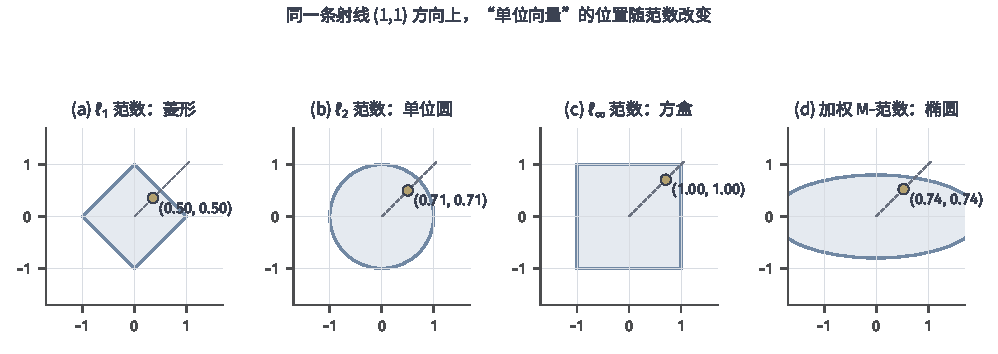
\includegraphics[width=169mm]{figures/00-shared/mathematical-preliminaries-upper/02-linear-spaces/matplotlib/ls-norm-unit-balls/ls-norm-unit-balls.pdf}
  \caption{同一向量在不同范数下的“单位球”形状。左：$\ell_1$单位球为菱形（累加绝对偏差）；中：$\ell_2$单位球为圆（欧氏长度）；右：$\ell_\infty$单位球为正方形（最大坐标偏差）。同一个点$(1,1)$的范数依次为$2$、$\sqrt2$、$1$，单位球大小随口径而变，三者之间的倍数关系将在第~\ref{sec:ls-norms-distances}节给出。三图坐标尺度相同，为解析教学例。}
  \label{fig:ls-norm-unit-balls}
\end{figure*}

本节建立了坐标向量的基本计算：加法、数乘与线性组合产生新的向量，欧氏内积把两个向量配成一个数，常用范数度量向量的大小。加法与数乘的规则将用于定义线性空间；内积与范数的一般性质留到第~\ref{chap:normed-inner-product-spaces}章。把若干向量并排放在一起，就得到下一节的矩阵。

% 第4章第2节（上）：矩阵的表示（矩阵、元素与形状，设计矩阵与贯穿例）、常见矩阵（方阵、零矩阵、对角矩阵、单位矩阵、上三角矩阵、下三角矩阵、对称矩阵、正定矩阵与半正定矩阵、置换矩阵、正交矩阵）、矩阵的运算（加法与数乘、转置、矩阵与向量的乘积、矩阵乘法、逐项乘积、逆矩阵、矩阵幂、迹、Frobenius内积、Frobenius范数、诱导矩阵范数、行列式）。运算性质随各项运算一并讨论。

\section{矩阵}
\label{sec:ls-matrices}

一批样本的特征排成一张数表以后，问题随之而来：对每个样本用同一组权重求加权和，要算许多个同样形式的和，能否一次写出；两次这样的计算接连进行，能否合成一次；一次计算能否撤销，反复进行时怎样书写；一张表把单位正方形变成平行四边形时，面积放大多少；作为计算，它最多把输入放大多少倍。这些问题都以矩阵为对象。本节先规定矩阵的写法，再介绍元素分布有固定模式的几类常见矩阵，然后逐一定义矩阵的运算，最后按运算整理它们满足的性质。

与向量不同，矩阵最重要的运算不是逐项进行的加法，而是由加权求和导出的乘法。乘法的规则与实数乘法有同有异，需要逐条核对。

\subsection{矩阵的表示与常见矩阵}
\label{sec:ls-matrix-representation}

定位向量中的一个数需要一个索引；一张数表的每个数要由所在的行与列共同确定，需要两个索引。

\paragraph{矩阵、元素与形状}
$m$行$d$列的实数表称为矩阵（matrix），记为$\bm A\in\mathbb R^{m\times d}$；第$i$行、第$j$列的元素记为$\bm A_{i,j}$，不会混淆时也写作$a_{i,j}$。$m\times d$称为矩阵的形状，行数写在列数之前。记号$\bm A_{i,:}$表示第$i$行，$\bm A_{:,j}$表示第$j$列，冒号表示该方向上的全部位置；第$j$列是一个$m$维列向量，第$i$行是一个$d$维行向量。例如在
\[
 \bm A=\begin{bmatrix}1&2&3\\4&5&6\end{bmatrix}\in\mathbb R^{2\times3}
\]
中，$\bm A_{2,1}=4$，第一行$\bm A_{1,:}=\left[\begin{smallmatrix}1&2&3\end{smallmatrix}\right]$，第三列$\bm A_{:,3}=(3,6)^\top$。

两个矩阵相等，要求形状相同且每个对应元素相等。只有一行的矩阵就是行向量，只有一列的矩阵就是列向量，所以向量可以看作矩阵的特例。

\paragraph{设计矩阵}
用矩阵记录数据时，通常让每行对应一个样本，每列对应一个特征，这样的矩阵称为设计矩阵。把示例~\ref{ex:ls-nearly-collinear-features}中两个特征的取值向量$\bm c_1,\bm c_2$并排作为两列，得到三个样本、两个特征的设计矩阵
\begin{equation}
\begin{gathered}
\bm X_{\varepsilon}
 =\begin{bmatrix}1&1\\1&1+\varepsilon\\1&1-\varepsilon\end{bmatrix}
 =\begin{bmatrix}\bm c_1&\bm c_2\end{bmatrix}\\
\bm q=\begin{bmatrix}0\\1\\-1\end{bmatrix},
 \quad \bm c_2=\bm c_1+\varepsilon\bm q.
\end{gathered}
\label{eq:linear-algebra-nearly-collinear-design}
\end{equation}
$|\varepsilon|$很小时，两列之差$\bm c_2-\bm c_1=\varepsilon\bm q$很短，两列几乎是同一串数；第~\ref{sec:ls-inner-product-definition}节将用夹角说明它们几乎同向。这个例子将贯穿整个线性空间部分：第~\ref{chap:linear-representation}章讨论这样两列能否充当一组记录方向，后面的谱与方程两章再看它怎样影响谱、求解与误差。

\subsubsection{常见矩阵}
\label{sec:prelim-common-matrices}

有些矩阵的元素分布有固定模式：大部分位置为零，或者主对角线两侧互相对称。这些模式会让后面的运算大为简化。本小节按元素的位置与取值逐类给出定义和例子；下面随各项运算讨论这些模式如何保留或改变；依赖内积的正交矩阵与正定矩阵在内积空间章建立。

\paragraph{方阵}
行数等于列数的矩阵称为方阵（square matrix），$n\times n$方阵也称$n$阶方阵；位置$(i,i)$上的元素组成主对角线。例如$\left[\begin{smallmatrix}1&2\\3&4\end{smallmatrix}\right]$是二阶方阵，主对角元素为$1$和$4$；$2\times3$矩阵不是方阵；这里讨论三角结构和对角矩阵时均限定为方阵。

\paragraph{零矩阵}
全部元素都为$0$的矩阵称为零矩阵（zero matrix），记作$\bm0$。它不要求是方阵，使用时须写明形状，例如
\[
 \bm0_{2\times3}=\begin{bmatrix}0&0&0\\0&0&0\end{bmatrix}.
\]

\paragraph{对角矩阵}
主对角线以外的元素都为$0$的方阵称为对角矩阵（diagonal matrix），记为$\operatorname{diag}(d_1,\ldots,d_n)$，主对角元素本身可以为$0$。例如
\[
\begin{gathered}
\operatorname{diag}(2,0)=\begin{bmatrix}2&0\\0&0\end{bmatrix}\\
\operatorname{diag}(1,-1,3)=\begin{bmatrix}1&0&0\\0&-1&0\\0&0&3\end{bmatrix}.
\end{gathered}
\]

\paragraph{单位矩阵}
主对角元素全为$1$的对角矩阵称为单位矩阵（identity matrix），记为$\bm I_n$，不必强调阶数时写作$\bm I$。它的第$j$列就是标准坐标向量$\bm e_j$。例如
\[
 \bm I_3=\begin{bmatrix}1&0&0\\0&1&0\\0&0&1\end{bmatrix}=\begin{bmatrix}\bm e_1&\bm e_2&\bm e_3\end{bmatrix}.
\]

\paragraph{上三角矩阵}
$i>j$时$\bm A_{i,j}=0$的方阵称为上三角矩阵（upper triangular matrix）：主对角线以下全为零，非零元素只可能出现在主对角线及其上方。例如
\[
 \begin{bmatrix}1&2&3\\0&4&5\\0&0&6\end{bmatrix}.
\]

\paragraph{下三角矩阵}
$i<j$时$\bm A_{i,j}=0$的方阵称为下三角矩阵（lower triangular matrix）：主对角线以上全为零。例如
\[
 \begin{bmatrix}1&0&0\\2&3&0\\4&5&6\end{bmatrix}.
\]
对角矩阵既是上三角矩阵，也是下三角矩阵。

\paragraph{对称矩阵}
满足$\bm A_{i,j}=\bm A_{j,i}$对全部$i,j$成立的方阵称为对称矩阵（symmetric matrix），它关于主对角线镜像对称；定义转置以后，这个条件写作$\bm A^\top=\bm A$。例如
\[
\begin{bmatrix}1&2\\2&3\end{bmatrix},\qquad
\begin{bmatrix}4&-1&0\\-1&2&5\\0&5&1\end{bmatrix}.
\]
对角矩阵都是对称矩阵。

\paragraph{置换矩阵}
把单位矩阵的各列重新排列得到的方阵称为置换矩阵（permutation matrix），它的每行、每列恰有一个$1$，其余为$0$。例如
\[
\begin{bmatrix}0&1\\1&0\end{bmatrix}=\begin{bmatrix}\bm e_2&\bm e_1\end{bmatrix},\qquad
\begin{bmatrix}0&0&1\\1&0&0\\0&1&0\end{bmatrix}=\begin{bmatrix}\bm e_2&\bm e_3&\bm e_1\end{bmatrix}.
\]
第一个矩阵乘在平面向量上会交换两个坐标，这一点在定义矩阵乘法以后验证。

\subsection{矩阵的基本运算}
\label{sec:ls-matrix-operation-properties}
\label{sec:ls-matrix-operations}
\label{sec:ls-multiplication}

矩阵的运算按来源可以分成几类。加法与数乘沿用向量的逐项规则，转置只改变元素的位置。矩阵与向量的乘积一次写出许多加权和，矩阵乘法、逆矩阵与矩阵幂都以它为基础。逐项乘积是另一种“相乘”，它不汇总任何索引。迹、行列式与矩阵范数把矩阵读成一个数，我们在下一节讨论。本节先给出运算方法，再检查它们满足的规则。

\subsubsection{加法与数乘}

同形矩阵$\bm A,\bm B\in\mathbb R^{m\times n}$逐项相加减，数乘把每个元素乘以同一个实数$c$：
\[
 \begin{gathered}
(\bm A\pm\bm B)_{i,j}=a_{i,j}\pm b_{i,j}\\
(c\bm A)_{i,j}=ca_{i,j},
 \end{gathered}
\]
结果形状不变。下面是一组二阶矩阵的算例。
\begin{example}[矩阵的加法、减法与数乘]
\label{ex:ls-matrix-addition-scaling}
给定：$\bm A=\left(\begin{smallmatrix}1&2\\3&4\end{smallmatrix}\right)$，$\bm B=\left(\begin{smallmatrix}0&1\\-1&2\end{smallmatrix}\right)$，$c=3$。
计算：逐项运算，
\[
\begin{gathered}
\bm A+\bm B=\begin{pmatrix}1&3\\2&6\end{pmatrix}\\
\bm A-\bm B=\begin{pmatrix}1&1\\4&2\end{pmatrix}\\
3\bm A=\begin{pmatrix}3&6\\9&12\end{pmatrix}.
\end{gathered}
\]
例如$\bm A+\bm B$的$(2,1)$元为$3+(-1)=2$，$\bm A-\bm B$的$(2,1)$元为$3-(-1)=4$。
结论：三个结果都是$2\times2$矩阵，每个元素只用到输入在同一位置上的元素。
\end{example}
与向量一样，两个矩阵能够相加，要求形状相同、对应位置含义相同；即使元素总数恰好相同，$2\times3$矩阵与$3\times2$矩阵也不能相加。同形矩阵的线性组合按同样方式定义。

\paragraph{加法与数乘的性质}

同形矩阵逐项相加与数乘，向量一节的八条规则在每个位置上照搬过来。对同形矩阵$\bm A,\bm B,\bm C$和实数$a,b$：
\[
\begin{aligned}
 &\bm A+\bm B=\bm B+\bm A, && (\bm A+\bm B)+\bm C=\bm A+(\bm B+\bm C),\\
 &\bm A+\bm0=\bm A, && \bm A+(-\bm A)=\bm0,\\
 &a(b\bm A)=(ab)\bm A, && 1\bm A=\bm A,\\
 &(a+b)\bm A=a\bm A+b\bm A, && a(\bm A+\bm B)=a\bm A+a\bm B.
\end{aligned}
\]
每一条都可以在任一位置$(i,j)$上用实数运算直接验证。


\subsubsection{转置}

转置交换行与列：$\bm A\in\mathbb R^{m\times n}$的元素$a_{i,j}$原样搬到$\bm A^\top\in\mathbb R^{n\times m}$的位置$(j,i)$，
\[
 (\bm A^\top)_{j,i}=\bm A_{i,j}.
\]
形状交换而数值不变，原来的第$i$行成为第$i$列。把列向量看作$d\times1$矩阵，这一定义与上一节向量的转置一致。下面的例子显示行怎样变成列。
\begin{example}[转置一个$2\times3$矩阵]
\label{ex:ls-transpose-two-by-three}
给定：$\bm A=\left[\begin{smallmatrix}1&2&3\\4&5&6\end{smallmatrix}\right]\in\mathbb R^{2\times3}$。
计算：把每个$(i,j)$元搬到$(j,i)$位置，
\[
 \bm A^\top=\begin{bmatrix}1&4\\2&5\\3&6\end{bmatrix}\in\mathbb R^{3\times2}.
\]
结论：$\bm A$的第一行$(1,2,3)$成为$\bm A^\top$的第一列，第二行$(4,5,6)$成为第二列。
\end{example}

\paragraph{转置的性质}
\label{sec:ls-reshaping}

转置改变元素的位置，也与其他矩阵运算有确定的关系。下面分别检查加法、数乘和乘积。

\paragraph{与加法、数乘交换}
\[
 \begin{gathered}
(\bm A+\bm B)^\top=\bm A^\top+\bm B^\top\\
(c\bm A)^\top=c\bm A^\top\\
(\bm A^\top)^\top=\bm A.
 \end{gathered}
\]
转置只搬动元素，逐项运算的结果搬到新位置后不变；转置两次，每个元素回到原来的位置。

\paragraph{乘积的转置}
\[
 (\bm A\bm B)^\top=\bm B^\top\bm A^\top.
\]
乘积转置后因子次序反转。按元素公式，
\[
 \begin{aligned}
 \bigl((\bm A\bm B)^\top\bigr)_{i,j}
 &=(\bm A\bm B)_{j,i}\\
 &=\sum_\ell a_{j,\ell}b_{\ell,i}\\
 &=\sum_\ell(\bm B^\top)_{i,\ell}(\bm A^\top)_{\ell,j}\\
 &=(\bm B^\top\bm A^\top)_{i,j}.
 \end{aligned}
\]
多个因子时依次使用，$(\bm A\bm B\bm C)^\top=\bm C^\top\bm B^\top\bm A^\top$。

\paragraph{内积中的转置}
\[
\langle\bm A\bm x,\bm y\rangle=\langle\bm x,\bm A^\top\bm y\rangle,\qquad
\bm A\in\mathbb R^{m\times d},\ \bm x\in\mathbb R^d,\ \bm y\in\mathbb R^m.
\]
由上一条，$(\bm A\bm x)^\top\bm y=\bm x^\top\bm A^\top\bm y$：在欧氏内积中，作用在左侧向量上的$\bm A$可以改写成作用在右侧向量上的$\bm A^\top$。

\paragraph{$\bm A^\top\bm A$对称}
对任意矩阵$\bm A$，$\bm A^\top\bm A$与$\bm A\bm A^\top$都是对称矩阵，因为$(\bm A^\top\bm A)^\top=\bm A^\top(\bm A^\top)^\top=\bm A^\top\bm A$，另一个同理。下面直接算出一个$\bm A\bm A^\top$。
\begin{example}[计算$\bm A\bm A^\top$]
\label{ex:ls-gram-product-symmetric}
给定：$\bm A=\left[\begin{smallmatrix}1&2&3\\4&5&6\end{smallmatrix}\right]$。
计算：$\bm A\bm A^\top$的$(i,j)$元是$\bm A$的第$i$行与第$j$行的内积，
\[
 \bm A\bm A^\top=\begin{bmatrix}1+4+9&4+10+18\\4+10+18&16+25+36\end{bmatrix}=\begin{bmatrix}14&32\\32&77\end{bmatrix}.
\]
结论：两个非对角元都是两行的内积$32$，结果是对称矩阵。
\end{example}

\subsubsection{矩阵与向量的乘积}
\label{sec:prelim-matrix-records-prediction}

设$n$次观测的输入排成设计矩阵$\bm X\in\mathbb R^{n\times d}$，权重排成$\bm w\in\mathbb R^d$。线性预测对每次观测计算同一种加权和$\sum_j x_{i,j}w_j$，即$\bm X$的第$i$行与$\bm w$的内积。矩阵与向量的乘积把这$n$个加权和一次写出：对$\bm A\in\mathbb R^{m\times d}$与$\bm u\in\mathbb R^d$，$\bm A\bm u$是$m$维列向量，
\begin{equation}
\begin{gathered}
(\bm A\bm u)_i=\sum_{j=1}^d\bm A_{i,j}u_j\\
i=1,\ldots,m.
\end{gathered}
\label{eq:prelim-matrix-prediction}
\end{equation}
矩阵的列数必须等于向量的维数。同一个结果有两种算法：
\begin{itemize}
 \item 按行算：输出的第$i$个坐标是第$i$行与$\bm u$的内积；
 \item 按列算：同一个$u_j$乘的恰好是第$j$列的全部元素，所以
 \[
  \bm A\bm u=u_1\bm A_{:,1}+u_2\bm A_{:,2}+\cdots+u_d\bm A_{:,d},
 \]
 乘积是矩阵各列以$u_j$为系数的线性组合。
\end{itemize}
特别地，按列算时，$\bm e_j$只有第$j$个系数为$1$，所以$\bm A\bm e_j=\bm A_{:,j}$：乘第$j$个标准坐标向量就取出第$j$列。

下面用一个二阶例子核对两种算法给出同一结果。
\begin{example}[按行与按列计算矩阵与向量的乘积]
\label{ex:ls-matrix-vector-rows-columns}
给定：$\bm A=\left[\begin{smallmatrix}2&1\\0&3\end{smallmatrix}\right]$，$\bm u=(1,1)^\top$。
计算：按行算，每个坐标是一行与$\bm u$的内积；按列算，结果是两列以$u_1=u_2=1$为系数的线性组合：
\[
\begin{gathered}
\bm A\bm u
 =\begin{bmatrix}2\cdot1+1\cdot1\\0\cdot1+3\cdot1\end{bmatrix}
 =\begin{bmatrix}3\\3\end{bmatrix}\\
\bm A\bm u=1\begin{bmatrix}2\\0\end{bmatrix}+1\begin{bmatrix}1\\3\end{bmatrix}
 =\begin{bmatrix}3\\3\end{bmatrix}.
\end{gathered}
\]
结论：两种算法都得到$\bm A\bm u=(3,3)^\top$。
\end{example}

用于数据时，矩阵与向量的乘积一次给出全部样本的预测。下面以一次函数为例。
\begin{example}[用矩阵与向量的乘积计算一次函数的取值]
\label{ex:ls-affine-predictions}
给定：要在$x=1,2,3$处计算$ax+b$，取
\[
\bm X=\begin{pmatrix}1&1\\2&1\\3&1\end{pmatrix},\qquad
\bm w=\begin{pmatrix}a\\b\end{pmatrix}.
\]
计算：按行算，
\[
 \bm X\bm w=\begin{pmatrix}1\cdot a+1\cdot b\\2\cdot a+1\cdot b\\3\cdot a+1\cdot b\end{pmatrix}=\begin{pmatrix}a+b\\2a+b\\3a+b\end{pmatrix}.
\]
结论：$\bm X\bm w$的三个坐标正是三处的函数值。第二列全为$1$，使每行都加上同一个截距$b$。
\end{example}

观测输出排成$\bm y$以后，全部残差就是$\bm X\bm w-\bm y$，平方误差总和写成
\[
 \sum_{i=1}^n\left(\sum_{j=1}^d x_{i,j}w_j-y_i\right)^2
 =\lVert\bm X\bm w-\bm y\rVert_2^2.
\]
左侧逐个样本求加权和、减去观测、平方后相加；右侧把同样的计算写成残差向量长度的平方。对贯穿例，按列算得$\bm X_\varepsilon\bm w=w_1\bm c_1+w_2\bm c_2$：预测是两个特征取值向量的线性组合。

\subsubsection{矩阵乘法}
\phantomsection
\label{sec:prelim-linear-actions-composition}

对$\bm A\in\mathbb R^{m\times d}$与$\bm B\in\mathbb R^{d\times k}$，乘积$\bm A\bm B\in\mathbb R^{m\times k}$为
\begin{equation}
 (\bm A\bm B)_{i,j}=\sum_{\ell=1}^d\bm A_{i,\ell}\bm B_{\ell,j}.
 \label{eq:prelim-matrix-composition}
\end{equation}
左矩阵的列数必须等于右矩阵的行数；第$(i,j)$项取左矩阵的第$i$行与右矩阵的第$j$列，逐项相乘后相加。下面逐项计算一个二阶乘积。
\begin{example}[二阶矩阵的乘积]
\label{ex:ls-matrix-product-2x2}
给定：$\bm A=\left(\begin{smallmatrix}1&1\\0&1\end{smallmatrix}\right)$，$\bm B=\left(\begin{smallmatrix}1&0\\0&2\end{smallmatrix}\right)$。
计算：第$(i,j)$项是$\bm A$的第$i$行与$\bm B$的第$j$列的内积，
\[
 \bm A\bm B
 =\begin{pmatrix}1\cdot1+1\cdot0&1\cdot0+1\cdot2\\0\cdot1+1\cdot0&0\cdot0+1\cdot2\end{pmatrix}
 =\begin{pmatrix}1&2\\0&2\end{pmatrix}.
\]
结论：$\bm A\bm B=\left(\begin{smallmatrix}1&2\\0&2\end{smallmatrix}\right)$，形状为$2\times2$。
\end{example}
$\bm B$只有一列时，式~\eqref{eq:prelim-matrix-composition}就是式~\eqref{eq:prelim-matrix-prediction}。两个向量的内积$\bm x^\top\bm y$是$1\times d$与$d\times1$矩阵的乘积，结果是$1\times1$矩阵，我们把它与它唯一的元素等同看待。

这个定义来自两次加权求和的接连进行。

设$\bm x\in\mathbb R^k$，$\bm y=\bm B\bm x$、$\bm z=\bm A\bm y$，即先用$\bm B$再用$\bm A$，这是第~\ref{sec:prelim-map-operations}节意义下两个函数的复合。逐坐标代入并交换有限求和的次序，
\begin{equation}
 z_i=\sum_{\ell=1}^d a_{i,\ell}y_\ell
 =\sum_{\ell=1}^d a_{i,\ell}\sum_{j=1}^k b_{\ell,j}x_j
 =\sum_{j=1}^k\left(\sum_{\ell=1}^d a_{i,\ell}b_{\ell,j}\right)x_j,
 \label{eq:linear-algebra-matrix-product}
\end{equation}
括号中的数正是$(\bm A\bm B)_{i,j}$。所以$(\bm A\bm B)\bm x=\bm A(\bm B\bm x)$：直接用乘积作用，等于先用$\bm B$、再用$\bm A$作用。被求和的公共维数$d$就是被消去的中间结果$\bm y$的维数。

非方阵相乘时，写出每个输入和输出的形状尤其有用。以$2\times3$矩阵乘$3\times2$矩阵为例，
\[
 \begin{aligned}
 &\begin{pmatrix}1&2&0\\0&1&3\end{pmatrix}
 \begin{pmatrix}1&0\\2&1\\1&-1\end{pmatrix}\\
 &=\begin{pmatrix}1\cdot1+2\cdot2+0\cdot1&1\cdot0+2\cdot1+0\cdot(-1)\\
 0\cdot1+1\cdot2+3\cdot1&0\cdot0+1\cdot1+3\cdot(-1)\end{pmatrix}\\
 &=\begin{pmatrix}5&2\\5&-2\end{pmatrix}.
 \end{aligned}
\]
两个中间维数都是$3$，因此乘法有定义；输出保留左矩阵的$2$行和右矩阵的$2$列。若把其中一个$3$改为其他数，逐项配对便无法完成。

\paragraph{乘法的性质}
矩阵乘法保留结合律和分配律，但通常不满足交换律。下面逐项核对这些规则，同时检查矩阵形状是否相容。

\paragraph{单位乘}
\[
\bm I_m\bm A=\bm A=\bm A\bm I_d,\qquad
\bm A\in\mathbb R^{m\times d}.
\]
$\bm I_m$的第$i$行是$\bm e_i^\top$，它与$\bm A$的第$j$列相乘取出$a_{i,j}$；右乘同理。单位矩阵在矩阵乘法中的作用相当于数$1$在实数乘法中的作用。

\paragraph{零乘}
\[
 \begin{gathered}
\bm0\bm A=\bm0\\
\bm A\bm0=\bm0.
 \end{gathered}
\]
乘积的每个元素都是若干乘积之和，其中一个因子全为零时，每一项都为零。这里各个零矩阵的形状由相乘的另一个因子决定。

反过来不成立：$\bm A\bm B=\bm0$不能推出$\bm A=\bm0$或$\bm B=\bm0$，下面是一个反例。
\begin{example}[反例：两个非零矩阵的乘积为零]
\label{ex:ls-zero-product-nonzero-factors}
给定：$\bm A=\left[\begin{smallmatrix}1&0\\0&0\end{smallmatrix}\right]$，$\bm B=\left[\begin{smallmatrix}0&0\\1&0\end{smallmatrix}\right]$，两者都不是零矩阵。
计算：
\[
 \bm A\bm B=\begin{bmatrix}1\cdot0+0\cdot1&1\cdot0+0\cdot0\\0\cdot0+0\cdot1&0\cdot0+0\cdot0\end{bmatrix}=\begin{bmatrix}0&0\\0&0\end{bmatrix}.
\]
结论：$\bm A\bm B=\bm0$，而$\bm A\neq\bm0$、$\bm B\neq\bm0$。
\end{example}
原因可以按列看出。由乘积的元素公式，$\bm A\bm B$的第$j$列就是$\bm A$乘$\bm B$的第$j$列，所以$\bm A\bm B=\bm0$恰好意味着$\bm B$的每一列$\bm b$都满足$\bm A\bm b=\bm0$：右因子产生的结果被左因子完全消去。上例中$\bm A$只保留第一个坐标、把第二个坐标清零，而$\bm B$的第一列$(0,1)^\top$只有第二个坐标非零，第二列为零。

\paragraph{结合律}
\[
 (\bm A\bm B)\bm C=\bm A(\bm B\bm C).
\]
按式~\eqref{eq:prelim-matrix-composition}展开，两边的第$(i,j)$项都是$\sum_k\sum_l a_{i,k}b_{k,l}c_{l,j}$，只是两个有限求和的次序不同。这也是函数复合满足结合律（第~\ref{sec:prelim-map-operations}节）在矩阵上的翻译。由结合律，多个相容矩阵连乘时不必标出括号。

\paragraph{分配律与数乘相容}
\[
 \begin{gathered}
\bm A(\bm B+\bm C)=\bm A\bm B+\bm A\bm C\\
(\bm A+\bm B)\bm C=\bm A\bm C+\bm B\bm C\\
c(\bm A\bm B)=(c\bm A)\bm B=\bm A(c\bm B),
 \end{gathered}
\]
逐项展开有限和即得。把右因子取为列向量，得到矩阵与向量的乘积对输入保持线性组合：
\begin{equation}
\bm A(a\bm u+b\bm v)=a\bm A\bm u+b\bm A\bm v,\qquad
\bm u,\bm v\in\mathbb R^d,\quad a,b\in\mathbb R.
\label{eq:prelim-matrix-linearity}
\end{equation}

由这一性质，函数$\bm u\mapsto\bm A\bm u$由它在$\bm e_1,\ldots,\bm e_d$上的输出完全确定：因为$\bm u=\sum_ju_j\bm e_j$，所以$\bm A\bm u=\sum_ju_j\bm A\bm e_j$，而这些输出$\bm A\bm e_j$就是$\bm A$的各列。第~\ref{chap:linear-representation}章把保持线性组合的函数称为线性映射，并说明每个这样的映射都能由一张矩阵记录。

\paragraph{分块乘法}
把矩阵按行、列分成尺寸相容的块，乘法规则对块照样成立：
\[
\begin{gathered}
\begin{bmatrix}\bm A&\bm B\end{bmatrix}\begin{bmatrix}\bm C\\\bm D\end{bmatrix}=\bm A\bm C+\bm B\bm D\\
\begin{bmatrix}\bm A\\\bm B\end{bmatrix}\bm C=\begin{bmatrix}\bm A\bm C\\\bm B\bm C\end{bmatrix},
\end{gathered}
\]
\[
 \bm A\begin{bmatrix}\bm C&\bm D\end{bmatrix}=\begin{bmatrix}\bm A\bm C&\bm A\bm D\end{bmatrix},
\]
以及$2\times2$分块的乘积
\[
 \begin{bmatrix}\bm A_{1,1}&\bm A_{1,2}\\\bm A_{2,1}&\bm A_{2,2}\end{bmatrix}
 \begin{bmatrix}\bm B_{1,1}&\bm B_{1,2}\\\bm B_{2,1}&\bm B_{2,2}\end{bmatrix}
 =\begin{bmatrix}
  \bm A_{1,1}\bm B_{1,1}+\bm A_{1,2}\bm B_{2,1}&\bm A_{1,1}\bm B_{1,2}+\bm A_{1,2}\bm B_{2,2}\\
  \bm A_{2,1}\bm B_{1,1}+\bm A_{2,2}\bm B_{2,1}&\bm A_{2,1}\bm B_{1,2}+\bm A_{2,2}\bm B_{2,2}
 \end{bmatrix}.
\]
条件是每个相乘的块对中，左块的列数等于右块的行数。第一式成立，是因为式~\eqref{eq:prelim-matrix-composition}对中间索引$\ell$的求和可以分段进行：前一段$\ell$对应$\bm A$的列与$\bm C$的行，后一段对应$\bm B$的列与$\bm D$的行，两段之和逐项等于整段求和。后两式只是把结果的行或列分组，$2\times2$分块由这三式合成。块可以像数一样参与运算，只是块之间的次序不能交换。

把块分到最细，得到三种常用的特例。右因子按列分块，得$(\bm A\bm B)_{:,j}=\bm A\bm B_{:,j}$：$\bm A$分别乘$\bm B$的每一列。左因子按行分块，得$(\bm A\bm B)_{i,:}=\bm A_{i,:}\bm B$：结果的第$i$行是$\bm B$各行以$\bm A_{i,:}$的元素为系数的线性组合。

第三种特例把中间维数$d$分成长度为$1$的$d$段，这时第一式给出
\begin{equation}
 \bm A\bm B=\sum_{\ell=1}^d\bm A_{:,\ell}\bm B_{\ell,:},
 \label{eq:ls-product-outer-sum}
\end{equation}
其中一列$\bm A_{:,\ell}\in\mathbb R^{m\times1}$乘一行$\bm B_{\ell,:}\in\mathbb R^{1\times k}$，得到$(i,j)$元素为$a_{i,\ell}b_{\ell,j}$的$m\times k$矩阵。式~\eqref{eq:ls-product-outer-sum}是后面低秩近似的出发点。下面用示例~\ref{ex:ls-matrix-product-2x2}的乘积核对这个公式。
\begin{example}[把乘积写成列乘行之和]
\label{ex:ls-product-as-outer-sum}
给定：示例~\ref{ex:ls-matrix-product-2x2}中的$\bm A=\left(\begin{smallmatrix}1&1\\0&1\end{smallmatrix}\right)$与$\bm B=\left(\begin{smallmatrix}1&0\\0&2\end{smallmatrix}\right)$。
计算：$\bm A$的两列为$(1,0)^\top$与$(1,1)^\top$，$\bm B$的两行为$(1,0)$与$(0,2)$，
\[
 \bm A\bm B=\begin{pmatrix}1\\0\end{pmatrix}\begin{pmatrix}1&0\end{pmatrix}+\begin{pmatrix}1\\1\end{pmatrix}\begin{pmatrix}0&2\end{pmatrix}
 =\begin{pmatrix}1&0\\0&0\end{pmatrix}+\begin{pmatrix}0&2\\0&2\end{pmatrix}=\begin{pmatrix}1&2\\0&2\end{pmatrix}.
\]
结论：两个“列乘行”矩阵之和与逐项计算的乘积相同。
\end{example}

\paragraph{交换律不成立}
一般$\bm A\bm B\neq\bm B\bm A$。形状不同时，两个乘积甚至不一定都有定义；即使两个因子是同阶方阵，两种次序的乘积也可能不同，下面是一个反例。
\begin{example}[反例：先交换再保留与先保留再交换]
\label{ex:ls-noncommuting-pair}
给定：只保留第一个坐标的$\bm P=\left[\begin{smallmatrix}1&0\\0&0\end{smallmatrix}\right]$，交换两个坐标的$\bm S=\left[\begin{smallmatrix}0&1\\1&0\end{smallmatrix}\right]$。
计算：
\[
\begin{gathered}
\bm P\bm S=\begin{bmatrix}0&1\\0&0\end{bmatrix}\\
\bm S\bm P=\begin{bmatrix}0&0\\1&0\end{bmatrix}.
\end{gathered}
\]
结论：$\bm P\bm S\neq\bm S\bm P$。作用在$\bm u\in\mathbb R^2$上，$\bm P\bm S\bm u=(u_2,0)^\top$是先交换、再保留第一个坐标，$\bm S\bm P\bm u=(0,u_1)^\top$是先保留、再交换，两种次序的结果不同。
\end{example}
书写$\bm A\bm B\bm x$时，作用顺序是从右向左：先$\bm B$，后$\bm A$。

\paragraph{消去律不成立}
$\bm A\bm B=\bm A\bm C$且$\bm A\neq\bm0$不能推出$\bm B=\bm C$。原因是$\bm A\bm B=\bm A\bm C$等价于$\bm A(\bm B-\bm C)=\bm0$，而乘积为零不能推出$\bm B-\bm C=\bm0$。下面用示例~\ref{ex:ls-zero-product-nonzero-factors}构造反例。
\begin{example}[反例：非零的左因子不能消去]
\label{ex:ls-cancellation-fails}
给定：示例~\ref{ex:ls-zero-product-nonzero-factors}中的$\bm A=\left[\begin{smallmatrix}1&0\\0&0\end{smallmatrix}\right]$与$\bm B=\left[\begin{smallmatrix}0&0\\1&0\end{smallmatrix}\right]$，以及$\bm C=\bm0$。
验证：$\bm A\bm B=\bm0=\bm A\bm C$，而$\bm B\neq\bm C$。
结论：虽然$\bm A\bm B=\bm A\bm C$且$\bm A\neq\bm0$，却不能消去$\bm A$得到$\bm B=\bm C$。
\end{example}
若$\bm A$是可逆方阵，在$\bm A\bm B=\bm A\bm C$两边左乘$\bm A^{-1}$即得$\bm B=\bm C$。所以左因子可逆时可以消去，一般的非零因子则不能。

常见矩阵参与乘法时，结果有固定模式。下面逐类给出。

\paragraph{对角矩阵的乘法}
对$\bm D=\operatorname{diag}(d_1,\ldots,d_n)$，
\[
 \begin{gathered}
(\bm D\bm A)_{i,j}=d_i\bm A_{i,j}\\
(\bm A\bm D)_{i,j}=\bm A_{i,j}d_j,
 \end{gathered}
\]
\[
 \operatorname{diag}(d_1,\ldots,d_n)\operatorname{diag}(e_1,\ldots,e_n)=\operatorname{diag}(d_1e_1,\ldots,d_ne_n).
\]
左乘对角矩阵缩放各行，右乘缩放各列：乘积公式中只有$\ell=i$（左乘时）或$\ell=j$（右乘时）的一项留下。作用在向量上，$\bm D\bm u=(d_1u_1,\ldots,d_nu_n)^\top$是逐坐标缩放。两个对角矩阵相乘时对角元逐个相乘，所以对角矩阵之间可以交换次序。下面的例子比较左乘与右乘。
\begin{example}[左乘与右乘对角矩阵]
\label{ex:ls-diagonal-scaling}
给定：$\bm D=\operatorname{diag}(2,3)$，$\bm A=\left[\begin{smallmatrix}1&2\\3&4\end{smallmatrix}\right]$。
计算：
\[
 \begin{aligned}
 \bm D\bm A&=\begin{bmatrix}2\cdot1&2\cdot2\\3\cdot3&3\cdot4\end{bmatrix}=\begin{bmatrix}2&4\\9&12\end{bmatrix},\\
 \bm A\bm D&=\begin{bmatrix}1\cdot2&2\cdot3\\3\cdot2&4\cdot3\end{bmatrix}=\begin{bmatrix}2&6\\6&12\end{bmatrix}.
 \end{aligned}
\]
结论：左乘把第一、二行分别乘以$2$、$3$，右乘把第一、二列分别乘以$2$、$3$。两个结果不同，所以对角矩阵与一般矩阵相乘时仍要区分左右。
\end{example}

\paragraph{三角矩阵的乘法}
若$\bm A,\bm B$都是$n$阶上三角矩阵，则$\bm A\bm B$也是上三角矩阵，并且
\[
 (\bm A\bm B)_{i,i}=\bm A_{i,i}\bm B_{i,i}.
\]
在$(\bm A\bm B)_{i,j}=\sum_\ell\bm A_{i,\ell}\bm B_{\ell,j}$中，$\bm A_{i,\ell}$只在$\ell\geq i$时可能非零，$\bm B_{\ell,j}$只在$\ell\leq j$时可能非零，所以只有$i\leq\ell\leq j$的项可能非零：$i>j$时没有这样的$\ell$，乘积元素为零；$i=j$时只剩$\ell=i$一项。下三角矩阵同理：两个下三角矩阵的乘积仍是下三角矩阵，对角元逐个相乘。下面是一个二阶算例。
\begin{example}[两个上三角矩阵的乘积]
\label{ex:ls-upper-triangular-product}
给定：$\bm A=\left[\begin{smallmatrix}1&2\\0&3\end{smallmatrix}\right]$，$\bm B=\left[\begin{smallmatrix}4&5\\0&6\end{smallmatrix}\right]$。
计算：
\[
 \bm A\bm B=\begin{bmatrix}1\cdot4+2\cdot0&1\cdot5+2\cdot6\\0\cdot4+3\cdot0&0\cdot5+3\cdot6\end{bmatrix}=\begin{bmatrix}4&17\\0&18\end{bmatrix}.
\]
结论：乘积仍是上三角矩阵，对角元$4=1\cdot4$、$18=3\cdot6$是两个因子对角元的乘积；右上角的$17$则同时用到了两个因子的非对角元。
\end{example}

\paragraph{置换矩阵的乘法}
设$\bm P=\left[\begin{smallmatrix}\bm e_{\sigma(1)}&\cdots&\bm e_{\sigma(n)}\end{smallmatrix}\right]$，其中$\sigma$是$\{1,\ldots,n\}$上的排列，则
\[
 \begin{gathered}
(\bm P\bm A)_{\sigma(i),:}=\bm A_{i,:}\\
(\bm A\bm P)_{:,j}=\bm A_{:,\sigma(j)}.
 \end{gathered}
\]
即左乘把$\bm A$的第$i$行移到第$\sigma(i)$行，右乘使$\bm A\bm P$的第$j$列取自$\bm A$的第$\sigma(j)$列。例如$\left[\begin{smallmatrix}0&1\\1&0\end{smallmatrix}\right]$左乘交换两行、右乘交换两列。

两个置换矩阵的乘积仍是置换矩阵：设$\bm P'$是另一个置换矩阵，$\bm P'\bm P$的第$j$列是$\bm P'\bm e_{\sigma(j)}$，即$\bm P'$的第$\sigma(j)$列；它是标准坐标向量，而且不同的$j$取到$\bm P'$的不同列，所以这些列互不相同。

\paragraph{对称矩阵的乘积}
若$\bm A,\bm B$是同阶对称矩阵，则
\[
 (\bm A\bm B)^\top=\bm B^\top\bm A^\top=\bm B\bm A,
\]
所以$\bm A\bm B$对称当且仅当$\bm A\bm B=\bm B\bm A$。对称矩阵的乘积一般不对称，下面是一个反例。
\begin{example}[反例：两个对称矩阵的乘积不对称]
\label{ex:ls-symmetric-product-not-symmetric}
给定：对称矩阵$\bm A=\left[\begin{smallmatrix}1&1\\1&0\end{smallmatrix}\right]$与$\bm B=\operatorname{diag}(1,2)$。
计算：右乘对角矩阵缩放各列，
\[
 \bm A\bm B=\begin{bmatrix}1\cdot1&1\cdot2\\1\cdot1&0\cdot2\end{bmatrix}=\begin{bmatrix}1&2\\1&0\end{bmatrix}.
\]
结论：$(\bm A\bm B)_{1,2}=2\neq1=(\bm A\bm B)_{2,1}$，乘积不对称。这与上面的判据一致：$\bm B\bm A=\left[\begin{smallmatrix}1&1\\2&0\end{smallmatrix}\right]\neq\bm A\bm B$。
\end{example}


\subsubsection{逐项乘积}
\label{sec:ls-hadamard-product}

矩阵乘法汇总共同索引；另一种常用的“乘法”不汇总任何索引，只把两个同形数组在对应位置配对。

设$\bm A,\bm B\in\mathbb R^{m\times n}$，\term{逐元素乘积}（Hadamard product）记作$\bm A\odot\bm B$，
\begin{equation}
 (\bm A\odot\bm B)_{i,j}=a_{i,j}b_{i,j},
 \label{eq:ls-hadamard}
\end{equation}
输出仍是$m\times n$。同维向量和更高阶的同形数组也按同样的方式逐项相乘。

同样两个矩阵，用两种乘法得到的结果完全不同，下面的例子说明这一点。
\begin{example}[逐项乘积与矩阵乘积的对比]
\label{ex:ls-hadamard-vs-matrix-product}
给定：$\bm A=\left[\begin{smallmatrix}1&2\\3&4\end{smallmatrix}\right]$，$\bm B=\left[\begin{smallmatrix}0&1\\1&0\end{smallmatrix}\right]$。
计算：
\[
 \begin{aligned}
 \bm A\odot\bm B&=\begin{bmatrix}1\cdot0&2\cdot1\\3\cdot1&4\cdot0\end{bmatrix}=\begin{bmatrix}0&2\\3&0\end{bmatrix},\\
 \bm A\bm B&=\begin{bmatrix}1\cdot0+2\cdot1&1\cdot1+2\cdot0\\3\cdot0+4\cdot1&3\cdot1+4\cdot0\end{bmatrix}=\begin{bmatrix}2&1\\4&3\end{bmatrix}.
 \end{aligned}
\]
结论：逐项乘积把$\bm B$为零的位置置零，矩阵乘积则交换了$\bm A$的两列；两个结果在每个位置上都不同。
\end{example}
固定掩码$\bm M$后，$\bm X\mapsto\bm M\odot\bm X$把$\bm M$为零的位置置零、把其余位置按系数缩放，适合表达“挑选或调制另一个数组”。

\paragraph{逐项乘积的性质}

逐项乘积的规则可以逐个位置从实数运算推出。以下矩阵的形状都相同。

\paragraph{交换律}
\[
 \bm A\odot\bm B=\bm B\odot\bm A.
\]
式~\eqref{eq:ls-hadamard}右端只是实数乘法，按位置逐项验证即得。逐项乘积可交换而矩阵乘积不可交换，再次说明两者是不同的运算。

\paragraph{结合律}
\[
 (\bm A\odot\bm B)\odot\bm C=\bm A\odot(\bm B\odot\bm C),
\]
两边的$(i,j)$元素都是$a_{i,j}b_{i,j}c_{i,j}$。

\paragraph{分配律}
\[
 \bm A\odot(\bm B+\bm C)=\bm A\odot\bm B+\bm A\odot\bm C,
\]
两边的$(i,j)$元素都是$a_{i,j}(b_{i,j}+c_{i,j})$。

\paragraph{单位元是全$1$数组}
全部元素为$1$的同形数组$\bm J$满足$\bm J\odot\bm A=\bm A$。单位矩阵不是逐项乘积的单位元：$\bm I_2\odot\bm A$只保留$\bm A$的对角元，把非对角元都变为零。

\paragraph{对每个因子分别线性}
固定一个因子时，$\bm X\mapsto\bm M\odot\bm X$保持线性组合。两个因子都作为未知量时，乘积只对各自分别线性：同时把两者放大两倍，结果放大四倍。第~\ref{chap:linear-representation}章换一组记录方向以后会看到，矩阵乘积对应的复合关系保持不变，逐项乘积则随记录方式改变。


\subsection{初等行变换与阶梯形}
\label{sec:ls-elementary-row-operations}

求逆时，我们需要把一个矩阵逐步化成容易辨认的形式。每一步都应当可以撤销，这样才不会丢失原矩阵中的信息。对矩阵的行允许三种\term{初等行变换}（elementary row operation）：交换两行；将一行乘以非零数；将一行加上另一行的倍数。它们的逆操作依次是再次交换同两行、乘以原系数的倒数，以及减去原来加上的倍数。

每种操作都可写成左乘一个初等矩阵：从单位矩阵出发，对其执行同样的行变换，所得矩阵记为$\bm E$，则$\bm E\bm A$恰好对$\bm A$执行该变换。例如交换两行的矩阵交换乘积的对应两行。逆操作也对应初等矩阵，因此$\bm E$可逆。

化简时从左到右寻找\term{主元}（pivot）。先在当前列尚未使用的行中找一个非零元素；若有必要，交换行把它移到当前行，再用它消去同列下方元素。若该列在余下各行全为零，就跳过这一列并继续向右。重复到没有可用行或列为止，得到的\term{行阶梯形}（row echelon form）中，零行位于底部，每个非零行的首个非零元位于上一行首个非零元的右侧。再把每个主元化为$1$，消去其上方元素，就得到\term{行最简形}（reduced row echelon form）。

处理方程$\bm A\bm x=\bm b$时，把右端项作为最后一列附在$\bm A$后面，得到增广矩阵$[\bm A\mid\bm b]$，并对整行执行同一操作。交换等式、将等式乘以非零数、把一个等式的倍数加到另一个等式，都不改变解；逆操作保证新的等式组也能还原为原等式组。下面在一个零候选主元和一列冗余的例子中逐步计算。
\begin{example}[换行、消元与自由变量]
\label{ex:ls-elementary-row-reduction}
考虑以下增广矩阵。第一列的首个元素为零，先交换前两行，再消去第三行的第一列：
\[
 \left[\begin{array}{ccc|c}0&1&2&3\\1&2&4&6\\2&4&8&12\end{array}\right]
 \longrightarrow
 \left[\begin{array}{ccc|c}1&2&4&6\\0&1&2&3\\2&4&8&12\end{array}\right]
 \longrightarrow
 \left[\begin{array}{ccc|c}1&2&4&6\\0&1&2&3\\0&0&0&0\end{array}\right].
\]
这已是阶梯形。将第一行减去第二行的两倍，得到行最简形
\[
 \left[\begin{array}{ccc|c}1&0&0&0\\0&1&2&3\\0&0&0&0\end{array}\right].
\]
第一、二列是主元列，第三列没有主元。令自由变量$x_3=t$，便读出$x_1=0$、$x_2=3-2t$；任意实数$t$都给出原方程组的一个解。最后的零行表示$0=0$，不会增加约束；若出现系数全为零而右端非零的行，则方程组无解。
\end{example}

阶梯形使主元和自由变量可见，但主元的选择会影响实际数值计算的误差。第~\ref{sec:ls-direct-methods}节会在求解方程时讨论选主元和计算代价。

\subsection{逆矩阵}
\label{sec:prelim-inverse-matrices}

对$n$阶方阵$\bm A$，若存在$n$阶方阵$\bm B$满足
\[
 \bm A\bm B=\bm B\bm A=\bm I_n,
\]
就称$\bm A$可逆，$\bm B$为\term{逆矩阵}（inverse matrix），记作$\bm A^{-1}$。逆矩阵撤销乘$\bm A$的效果。$\bm A$可逆时，若$\bm A\bm x=\bm y$，两边左乘$\bm A^{-1}$得$\bm x=\bm A^{-1}\bm y$，所以方程至多有一个解；反过来，$\bm x=\bm A^{-1}\bm y$满足$\bm A\bm x=\bm A\bm A^{-1}\bm y=\bm y$。所以方程$\bm A\bm x=\bm y$有唯一解$\bm x=\bm A^{-1}\bm y$。

逆矩阵若存在则唯一：若$\bm B,\bm C$都满足条件，则$\bm B=\bm B(\bm A\bm C)=(\bm B\bm A)\bm C=\bm C$，这里用到前面建立的结合律。因此记号$\bm A^{-1}$不会有歧义。

怎样求逆取决于矩阵的结构。下面从最简单的对角矩阵开始，依次给出二阶方阵的公式与一般方阵的做法。

\paragraph{对角矩阵的逆}
每个$d_i\neq0$时逐个取倒数：
\[
 \operatorname{diag}(d_1,\ldots,d_n)^{-1}=\operatorname{diag}(1/d_1,\ldots,1/d_n).
\]
两个对角矩阵相乘时对角元逐个相乘（前面已验证），所以两侧乘积都是$\bm I_n$。例如$\operatorname{diag}(2,1)^{-1}=\operatorname{diag}(1/2,1)$。若某个$d_i=0$，左乘$\bm D=\operatorname{diag}(d_1,\ldots,d_n)$把任何$\bm B$的第$i$行乘以$d_i$，所以$\bm D\bm B$的第$i$行是$\bm0$，不可能等于$\bm I_n$的第$i$行；这时$\bm D$不可逆。

\paragraph{二阶方阵的逆}
$ad-bc\neq0$时，
\[
 \begin{pmatrix}a&b\\c&d\end{pmatrix}^{-1}=\frac1{ad-bc}\begin{pmatrix}d&-b\\-c&a\end{pmatrix}.
\]
直接相乘即可验证两侧乘积都是$\bm I_2$：例如左上元素为$(ad-bc)/(ad-bc)=1$，右上元素为$(-ab+ba)/(ad-bc)=0$。分母$ad-bc$正是后面的二阶行列式。

\paragraph{一般方阵的逆}
一般方阵没有这样简短的公式，可以通过解方程求逆：对任意$\bm y$解$\bm A\bm x=\bm y$，把$\bm x$写成$\bm y$各坐标的线性组合，系数排成的矩阵就是$\bm A^{-1}$。下面用一个二阶例子演示，并与二阶公式对照。
\begin{example}[解方程求逆]
\label{ex:ls-inverse-by-solving}
给定：$\bm A=\left[\begin{smallmatrix}2&1\\0&3\end{smallmatrix}\right]$。
计算：方程$\bm A\bm x=\bm y$即$y_1=2x_1+x_2$、$y_2=3x_2$。由第二式得$x_2=y_2/3$，代入第一式得$x_1=(y_1-x_2)/2=y_1/2-y_2/6$。把系数排成矩阵，
\[
 \bm A^{-1}=\begin{bmatrix}1/2&-1/6\\0&1/3\end{bmatrix}.
\]
用二阶公式核对：$ad-bc=2\cdot3-1\cdot0=6$，公式给出$\frac16\left[\begin{smallmatrix}3&-1\\0&2\end{smallmatrix}\right]$，与上式相同。
结论：右上角的$-1/6$不是原元素$1$的倒数。一般矩阵把各个坐标掺在一起，逆矩阵要作为整体求出，不能逐个元素取倒数。
\end{example}
上述求法也可以用初等行变换同时处理所有右端项。把$\bm A$与单位矩阵并排，得到$[\bm A\mid\bm I_n]$，对整个增广矩阵作行变换。若左侧最终化为$\bm I_n$，这些操作合起来是某个可逆矩阵$\bm E$的左乘，于是$\bm E\bm A=\bm I_n$、右侧为$\bm E$，故$\bm E=\bm A^{-1}$。例如
\[
 \begin{aligned}
 &\left[\begin{array}{cc|cc}2&1&1&0\\0&3&0&1\end{array}\right]\\
 &\longrightarrow
 \left[\begin{array}{cc|cc}1&1/2&1/2&0\\0&1&0&1/3\end{array}\right]\\
 &\longrightarrow
 \left[\begin{array}{cc|cc}1&0&1/2&-1/6\\0&1&0&1/3\end{array}\right],
 \end{aligned}
\]
右半部分与前面的逆矩阵相同。如果方阵化简后不能在每列找到主元，左侧出现零行；由于所有行变换都可逆，这样的矩阵不能有逆。计算方程的解时，通常直接对右端项消元，不必先求出整个逆矩阵。哪些方阵可逆，第~\ref{sec:ls-injective-surjective-invertible}节用零空间与秩回答，第~\ref{sec:ls-determinant-invertibility}节再给出行列式判据。

\paragraph{单侧逆}
矩形矩阵不能有双侧的逆，但可能只从一侧抵消。对$\bm A\in\mathbb R^{m\times d}$，满足$\bm L\bm A=\bm I_d$的$\bm L\in\mathbb R^{d\times m}$称为左逆，满足$\bm A\bm R=\bm I_m$的$\bm R\in\mathbb R^{d\times m}$称为右逆。有左逆时，若$\bm A\bm x=\bm y$有解，两边左乘$\bm L$得$\bm x=\bm L\bm y$，所以解只能是$\bm L\bm y$。有右逆时，$\bm A(\bm R\bm y)=\bm I_m\bm y=\bm y$，所以$\bm x=\bm R\bm y$总是一个解。

与方阵的逆不同，单侧逆一般不唯一，下面的例子说明这一点。
\begin{example}[反例：左逆不唯一]
\label{ex:ls-left-inverse-not-unique}
给定：$\bm A=(1,0)^\top\in\mathbb R^{2\times1}$，以及任意实数$c$。
验证：取$\bm L=(1,c)\in\mathbb R^{1\times2}$，则$\bm L\bm A=1\cdot1+c\cdot0=1=\bm I_1$。
结论：每个$c$都给出$\bm A$的一个左逆，所以$\bm A$的左逆有无穷多个。
\end{example}
矩形矩阵何时有左逆或右逆，第~\ref{chap:linear-representation}章用核与像回答；第~\ref{chap:linear-equations-and-optimization}章讨论怎样实际求解，以及多解时选哪一个。

设下面的$\bm A,\bm B$都是$n$阶可逆方阵。

\paragraph{乘积的逆}
\begin{equation}
 (\bm A\bm B)^{-1}=\bm B^{-1}\bm A^{-1}.
 \label{eq:ls-inverse-product}
\end{equation}
先作用的后撤销，就像先穿袜子再穿鞋，脱的时候要先脱鞋。验证：$(\bm A\bm B)(\bm B^{-1}\bm A^{-1})=\bm A(\bm B\bm B^{-1})\bm A^{-1}=\bm A\bm A^{-1}=\bm I_n$，反方向$(\bm B^{-1}\bm A^{-1})(\bm A\bm B)=\bm I_n$同理。

\paragraph{逆的逆}
\[
 (\bm A^{-1})^{-1}=\bm A.
\]
定义中$\bm A$与$\bm A^{-1}$的地位对称：$\bm A^{-1}\bm A=\bm A\bm A^{-1}=\bm I_n$同样说明$\bm A$是$\bm A^{-1}$的逆。

\paragraph{数乘的逆}
\[
 (c\bm A)^{-1}=c^{-1}\bm A^{-1}\qquad(c\neq0).
\]
直接相乘：$(c\bm A)(c^{-1}\bm A^{-1})=(cc^{-1})\bm A\bm A^{-1}=\bm I_n$，反方向同理。

\paragraph{转置的逆}
\[
 (\bm A^\top)^{-1}=(\bm A^{-1})^\top.
\]
由乘积的转置，$\bm A^\top(\bm A^{-1})^\top=(\bm A^{-1}\bm A)^\top=\bm I^\top=\bm I$，反方向同理，所以$(\bm A^{-1})^\top$就是$\bm A^\top$的逆。

\subsection{矩阵的幂}
\label{sec:ls-matrix-power-rules}

定常迭代$\bm x^{(k+1)}=\bm A\bm x^{(k)}$每一步都乘同一个$\bm A$。对$d$阶方阵，$\bm A^k$定义为$k$个$\bm A$连乘（$k\geq1$），并规定$\bm A^0=\bm I_d$；$\bm A$可逆时再定义负幂$\bm A^{-k}=(\bm A^{-1})^k$。于是迭代的第$k$步是$\bm x^{(k)}=\bm A^k\bm x^{(0)}$。非方阵不能与自身相乘，所以没有矩阵幂。

幂是反复的矩阵乘法，不是逐元素乘方，下面的例子说明两者的差别。
\begin{example}[矩阵的平方不是逐元素平方]
\label{ex:ls-matrix-square-shear}
给定：$\bm A=\left(\begin{smallmatrix}1&1\\0&1\end{smallmatrix}\right)$。
计算：
\[
 \bm A^2=\begin{pmatrix}1&1\\0&1\end{pmatrix}\begin{pmatrix}1&1\\0&1\end{pmatrix}
 =\begin{pmatrix}1\cdot1+1\cdot0&1\cdot1+1\cdot1\\0\cdot1+1\cdot0&0\cdot1+1\cdot1\end{pmatrix}
 =\begin{pmatrix}1&2\\0&1\end{pmatrix}.
\]
结论：右上角的元素变为$2$，而逐元素平方会得到$1^2=1$；继续相乘，右上角每次增加$1$。
\end{example}

同一矩阵的整数幂按结合律满足$\bm A^r\bm A^s=\bm A^{r+s}$和$(\bm A^r)^s=\bm A^{rs}$；出现负指数时要求$\bm A$可逆。但不同矩阵不一定交换，因此
\[
 (\bm A+\bm B)^2=\bm A^2+\bm A\bm B+\bm B\bm A+\bm B^2,
\]
只有$\bm A\bm B=\bm B\bm A$时才能将中间两项合成$2\bm A\bm B$。这与标量平方公式的差别来自乘法次序。

两类幂关系经常出现。满足$\bm A^2=\bm A$的方阵称为\term{幂等}（idempotent）矩阵，乘一次与乘多次效果相同。存在正整数$s$使$\bm N^s=\bm0$的方阵称为\term{幂零}（nilpotent）矩阵。下面各举一例。
\begin{example}[幂等矩阵与幂零矩阵]
\label{ex:ls-idempotent-nilpotent}
给定：$\bm P=\operatorname{diag}(1,0)$，$\bm N=\left(\begin{smallmatrix}0&1\\0&0\end{smallmatrix}\right)$。
计算：对$\bm u\in\mathbb R^2$，$\bm P\bm u=(u_1,0)^\top$只保留第一个坐标，再作用一次结果不变，所以$\bm P^2=\bm P$。$\bm N\bm u=(u_2,0)^\top$把第二个坐标移到第一个位置、把第二个位置清零；再作用一次得$\bm N(u_2,0)^\top=(0,0)^\top$。直接相乘也得到
\[
 \bm N^2=\begin{pmatrix}0&1\\0&0\end{pmatrix}\begin{pmatrix}0&1\\0&0\end{pmatrix}=\begin{pmatrix}0&0\\0&0\end{pmatrix}.
\]
结论：$\bm P$是幂等矩阵；$\bm N\neq\bm0$，却满足$\bm N^2=\bm0$，是幂零矩阵。
\end{example}
$\bm A^k$在$k$很大时是什么样子，很难从元素看出，第~\ref{chap:linear-analysis}章借助特征向量回答。

\paragraph{幂的性质}

设$\bm A$为方阵，$m,n$为非负整数；$\bm A$可逆时，$m,n$可取任意整数。

\paragraph{同底幂相乘}
\[
 \bm A^m\bm A^n=\bm A^{m+n}.
\]
由结合律，两边都是同样个数的$\bm A$（或$\bm A^{-1}$）连乘；指数异号时，相邻的$\bm A\bm A^{-1}$逐对消去。交换$m,n$的角色可见，同一矩阵的不同次幂彼此可以交换。

\paragraph{幂的幂}
\[
 (\bm A^m)^n=\bm A^{mn}.
\]
左边是$n$组、每组$m$个因子的连乘，由结合律去掉括号即得。

\paragraph{负幂与逆相容}
\[
 (\bm A^k)^{-1}=(\bm A^{-1})^k=\bm A^{-k}.
\]
对$k$个相同因子反复使用式~\eqref{eq:ls-inverse-product}即得。

% 方阵和同形矩阵的标量读数：行列式、迹与元素内积。
\section{行列式、迹与元素内积}
\label{sec:ls-matrix-scalar-readouts}

矩阵运算可以产生另一张数表，也可以产生一个标量。行列式衡量方阵作用下有向体积的缩放；迹累计主对角元素；Frobenius内积比较同形矩阵的全部对应元素。它们回答的问题不同，不能只凭其中一个数恢复原矩阵。

\subsection{行列式的定义与计算}
\phantomsection
\label{sec:ls-exterior-determinants}
\label{sec:linear-algebra-scalar-readouts}

一张方阵把单位正方形变成平行四边形、把单位立方体变成平行多面体时，面积或体积放大多少倍？平行四边形的面积不能由两条边的长度直接算出，它还取决于两个向量的相对方向；若再记录定向，交换两个向量的次序会使有向面积变号。下面先建立记录有向体积的外积，再由它得到行列式和它的计算公式。

\paragraph{外积}
对$\mathbb R^d$中的$k$个向量$\bm v_1,\ldots,\bm v_k$，它们的\term{外积}（exterior product，又称\term{楔积}wedge product）$\bm v_1\wedge\cdots\wedge\bm v_k$按两条规则计算。
\begin{itemize}
 \item 多线性：对每个因子分别保持线性组合，即把某个$\bm v_i$换成$a\bm u+b\bm w$时，整个楔积等于$a(\cdots\wedge\bm u\wedge\cdots)+b(\cdots\wedge\bm w\wedge\cdots)$，其余因子不动。
 \item 交替性：交换相邻两个因子，楔积变号，
 \[
  \cdots\wedge\bm v_i\wedge\bm v_j\wedge\cdots
  =-\cdots\wedge\bm v_j\wedge\bm v_i\wedge\cdots.
 \]
\end{itemize}

两条规则先给出两个推论。第一，含有两个相同因子的楔积为零：两个相同因子相邻时，交换它们不改变楔积，却使它变号，所以它等于自身的相反数，只能为零；两个相同因子不相邻时，先用相邻交换把它们移到一起，只改变符号，结论不变。第二，若某个因子是其余因子的线性组合，把这个因子按组合代入并由多线性展开，每一项都含有两个相同因子，所以整个楔积为零。

由此可以确定楔积的一般形状。

设$v_{j,i}$是$\bm v_j$的第$i$个坐标，把每个$\bm v_j=\sum_i v_{j,i}\bm e_i$代入并展开，含重复下标的项为零；其余各项按交替性把下标排成递增次序，只改变符号。所以每个楔积都是基楔积$\bm e_{i_1}\wedge\cdots\wedge\bm e_{i_k}$（$i_1<\cdots<i_k$）的线性组合，这样的基楔积共有$\binom{d}{k}$个。$k>d$时，每一项都必然含有重复下标，所以楔积恒为零。

对$\{1,\ldots,k\}$上的一般排列$\pi$，可以反复交换相邻的两个因子，把$\bm v_{\pi(1)}\wedge\cdots\wedge\bm v_{\pi(k)}$排回$\bm v_1\wedge\cdots\wedge\bm v_k$。记$N(\pi)$为$\pi$的逆序对数，即满足$i<j$而$\pi(i)>\pi(j)$的索引对数。每次交换一对相邻且次序颠倒的因子，逆序对数恰好减少$1$，所以恰好经过$N(\pi)$次交换就排好，每次交换变号一次，得到
\[
 \begin{gathered}
\bm v_{\pi(1)}\wedge\cdots\wedge\bm v_{\pi(k)}
 =\operatorname{sgn}(\pi)\,\bm v_1\wedge\cdots\wedge\bm v_k\\
\operatorname{sgn}(\pi)=(-1)^{N(\pi)}.
 \end{gathered}
\]

\paragraph{有向面积与有向体积}
在$\mathbb R^2$中按两条规则展开，
\[
 \bm u\wedge\bm v
 =(u_1\bm e_1+u_2\bm e_2)\wedge(v_1\bm e_1+v_2\bm e_2)
 =(u_1v_2-u_2v_1)\,\bm e_1\wedge\bm e_2,
\]
其中用到$\bm e_1\wedge\bm e_1=\bm e_2\wedge\bm e_2=0$与$\bm e_2\wedge\bm e_1=-\bm e_1\wedge\bm e_2$。系数$u_1v_2-u_2v_1$是$\bm u,\bm v$张成的平行四边形的有向面积：绝对值是面积，符号是定向。

下面用三组向量观察有向面积的数值与符号。
\begin{example}[平面上的有向面积]
\label{ex:ls-oriented-area}
给定：三组有序向量对：$\bm u=(1,0)^\top$与$\bm v=(1,1)^\top$；交换次序后的$\bm v$与$\bm u$；共线的$(1,1)^\top$与$(2,2)^\top$。
计算：按系数公式$u_1v_2-u_2v_1$，三组依次得到
\[
 \begin{gathered}
1\cdot1-0\cdot1=1\\
1\cdot0-1\cdot1=-1\\
1\cdot2-1\cdot2=0.
 \end{gathered}
\]
结论：第一组张成面积为$1$的平行四边形；交换次序后面积不变而定向翻转，所以符号变负；共线的两个向量张成的平行四边形退化成线段，有向面积为$0$。
\end{example}
由上面的计数，$\mathbb R^3$中三个向量的楔积只是基楔积$\bm e_1\wedge\bm e_2\wedge\bm e_3$的倍数。这个系数的绝对值是三个向量张成的平行六面体的体积，带符号时称为\term{有向体积}。

\paragraph{行列式的定义}
在$\mathbb R^d$中取$d$个向量，最高阶楔积只剩一个基楔积$\bm e_1\wedge\cdots\wedge\bm e_d$。对$d$阶方阵$\bm A$，把它的各列$\bm A\bm e_1,\ldots,\bm A\bm e_d$作楔积，
\[
 \bm A\bm e_1\wedge\cdots\wedge\bm A\bm e_d
 =(\det\bm A)\,\bm e_1\wedge\cdots\wedge\bm e_d,
\]
标量$\det\bm A$称为\term{行列式}（determinant）。它是$\bm A$把单位立方体变成平行多面体时的有向体积倍数，绝对值为体积比，符号表示定向是否翻转。图~\ref{fig:ls-determinant-oriented-volume}在平面上画出这一缩放。
\begin{figure*}[htbp]
  \centering
  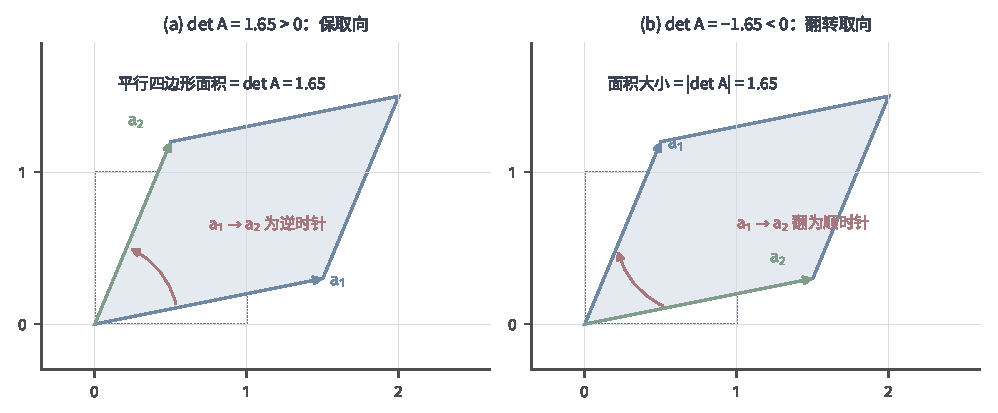
\includegraphics[width=169mm]{figures/00-shared/mathematical-preliminaries-upper/02-linear-spaces/matplotlib/ls-determinant-oriented-volume/ls-determinant-oriented-volume.pdf}
  \caption{行列式作为有向体积的缩放。左：单位正方形由$\bm e_1=(1,0)$、$\bm e_2=(0,1)$张成，面积为$1$。中：$\bm A=\bigl(\begin{smallmatrix}2&0.5\\0&1.5\end{smallmatrix}\bigr)$把它映成由$\bm A\bm e_1=(2,0)$、$\bm A\bm e_2=(0.5,1.5)$张成的平行四边形，有向面积为$2\cdot1.5-0.5\cdot0=3=\det\bm A>0$（保定向）。右：$\bm A$把$\bm e_1$反射到$(-2,0)$，有向面积为$-3$（反定向）。向量与数值均为解析教学例。}
  \label{fig:ls-determinant-oriented-volume}
\end{figure*}

\paragraph{排列展开}
把$\bm A\bm e_j=\sum_i a_{i,j}\bm e_i$代入楔积并展开。若第$j$个因子选出$\bm e_{\tau(j)}$，得到的项为$\bigl(\prod_ja_{\tau(j),j}\bigr)\,\bm e_{\tau(1)}\wedge\cdots\wedge\bm e_{\tau(d)}$。下标有重复的项为零；留下的项中$\tau$是$\{1,\ldots,d\}$的一个排列，而$\bm e_{\tau(1)}\wedge\cdots\wedge\bm e_{\tau(d)}=\operatorname{sgn}(\tau)\,\bm e_1\wedge\cdots\wedge\bm e_d$。所以
\[
 \det\bm A=\sum_{\tau}\operatorname{sgn}(\tau)\prod_{j=1}^d a_{\tau(j),j},
\]
求和遍历全部排列。习惯上按行书写：记$\pi=\tau^{-1}$，把乘积按行号重排，得到$\prod_ia_{i,\pi(i)}$。$\tau$的逆序对$(i,j)$与$\pi$的逆序对$(\tau(j),\tau(i))$一一对应，所以$\operatorname{sgn}(\pi)=\operatorname{sgn}(\tau)$。于是得到计算公式
\[
 \det\bm A
 =\sum_{\pi\in S_d}\operatorname{sgn}(\pi)
   \prod_{i=1}^d a_{i,\pi(i)},
\]
其中$S_d$是$\{1,\ldots,d\}$到自身的全部双射，每个$\pi$规定第$i$行选取第$\pi(i)$列。计算步骤是：对每个排列，从每行各取一个元素、各列恰好取一次，把取出的$d$个数相乘，再按逆序对数的奇偶加上正负号求和。

二阶时只有两个排列：恒等排列没有逆序对，取正号；交换$1,2$的排列有一个逆序对，取负号。于是
\[
 \det\begin{pmatrix}a&b\\c&d\end{pmatrix}=ad-bc,
\]
例如$\det\left(\begin{smallmatrix}1&2\\3&4\end{smallmatrix}\right)=1\cdot4-2\cdot3=-2$。

三阶时有六个排列。恒等排列与两个循环排列$(\pi(1),\pi(2),\pi(3))=(2,3,1)$、$(3,1,2)$的逆序对数为$0$或$2$，取正号；只交换两个位置的三个排列$(1,3,2)$、$(2,1,3)$、$(3,2,1)$的逆序对数为$1$或$3$，取负号。于是
\[
 \begin{aligned}
 \det\bm A={}&a_{1,1}a_{2,2}a_{3,3}+a_{1,2}a_{2,3}a_{3,1}+a_{1,3}a_{2,1}a_{3,2}\\
 &-a_{1,1}a_{2,3}a_{3,2}-a_{1,2}a_{2,1}a_{3,3}-a_{1,3}a_{2,2}a_{3,1}.
 \end{aligned}
\]
下面用这个公式计算一个具体的三阶行列式。
\begin{example}[三阶行列式的排列展开]
\label{ex:ls-det-three-by-three}
给定：$\bm A=\left(\begin{smallmatrix}2&0&1\\1&3&0\\0&1&1\end{smallmatrix}\right)$。
计算：按上式的六项次序代入，
\[
 \begin{aligned}
 \det\bm A&=2\cdot3\cdot1+0\cdot0\cdot0+1\cdot1\cdot1-2\cdot0\cdot1-0\cdot1\cdot1-1\cdot3\cdot0\\
 &=6+0+1-0-0-0=7.
 \end{aligned}
\]
结论：$\det\bm A=7$。六项中只有两项非零，其余四项都含有零元素。
\end{example}

行列式因而是矩阵元素的多项式。上面的推导只说明：若楔积满足两条规则，行列式只能是这个和。反过来可以直接验证，排列展开式作为各列的函数确实对每列线性、交换两列时变号（交换两列相当于把每个$\pi$复合上一次对换，逆序对数的奇偶随之改变），并且在单位矩阵处等于$1$。所以两条规则彼此相容，行列式由它们和$\det\bm I_d=1$唯一确定。高阶时排列有$d!$个，实际计算通常利用下面的性质和消元。



\subsection{行列式的性质与可逆性}
\label{sec:ls-determinant-properties}
\phantomsection
\label{sec:prelim-determinants}

行列式由楔积的两条规则定义，下面前两条性质就是这两条规则在列上的表述，其余性质由它们推出。

设$\bm A,\bm B$为$d$阶方阵。

\paragraph{对列的多线性}
\[
 \det\begin{bmatrix}\cdots&a\bm u+b\bm w&\cdots\end{bmatrix}
 =a\det\begin{bmatrix}\cdots&\bm u&\cdots\end{bmatrix}
 +b\det\begin{bmatrix}\cdots&\bm w&\cdots\end{bmatrix},
\]
其中三个矩阵只在同一列不同，其余各列相同。$\det\bm A$是各列楔积的系数，所以这正是楔积对每个因子保持线性组合的直接翻译。

\paragraph{交替性}
交换两列，行列式变号；两列相同，行列式为零。前者来自楔积交换两个因子时变号（不相邻的两个因子可以经奇数次相邻交换互换位置）；后者是因为交换两个相同的列不改变矩阵，行列式却要变号，只能为零。

两条合起来又得到两个常用推论。把某列的倍数加到另一列上，行列式不变：按多线性拆开，多出的一项含两列相同，为零。某一列是其余各列的线性组合时，行列式为零：把这一列按组合展开，每一项都含两列相同。例如$\det\left(\begin{smallmatrix}1&2\\2&4\end{smallmatrix}\right)=4-4=0$，第二列是第一列的$2$倍。

\paragraph{转置不变}
\[
 \det(\bm A^\top)=\det\bm A.
\]
在排列展开中，把每一项的乘积按列号重排，得$\prod_ia_{i,\pi(i)}=\prod_ja_{\pi^{-1}(j),j}$；排列展开的推导已经说明$\operatorname{sgn}(\pi^{-1})=\operatorname{sgn}(\pi)$。$\pi$遍历$S_d$时，$\sigma=\pi^{-1}$也遍历$S_d$，所以
\[
 \det\bm A=\sum_{\sigma\in S_d}\operatorname{sgn}(\sigma)\prod_{j=1}^da_{\sigma(j),j}
 =\sum_{\sigma\in S_d}\operatorname{sgn}(\sigma)\prod_{j=1}^d(\bm A^\top)_{j,\sigma(j)}
 =\det(\bm A^\top).
\]
于是对列成立的多线性与交替性，对行同样成立。

\paragraph{行变换与可逆性}
行上的多线性和交替性给出三条计算规则：交换两行使行列式变号；某行乘以非零数$c$使行列式乘以$c$；某行加上另一行的倍数不改变行列式。第三条是因为按该行展开后，多出的矩阵有两行相同，其行列式为零。

用这些规则配合消元，可以把方阵化为上三角矩阵，再取对角元素的乘积并补偿换行及倍乘的影响。例如
\[
 \det\begin{pmatrix}0&1&2\\1&2&1\\2&7&4\end{pmatrix}
 =-\det\begin{pmatrix}1&2&1\\0&1&2\\0&3&2\end{pmatrix}
 =-\det\begin{pmatrix}1&2&1\\0&1&2\\0&0&-4\end{pmatrix}=4.
\]
第一步交换前两行，并从第三行减去第一行的两倍；第二步再从第三行减去第二行的三倍。交换行使符号改变，两次加倍数不改变行列式。

这也把行列式与求逆联系起来。消元中的每一步都可逆，而且只使行列式乘以一个非零数。

若每列都找到主元，阶梯形是对角元非零的上三角矩阵，故行列式非零，并可继续化为单位矩阵求逆。

若某列找不到主元，方阵的阶梯形至少有一行全零，行列式为零，也无法化为单位矩阵。因此方阵可逆当且仅当其行列式非零。

\paragraph{数乘与加法}
\[
\begin{gathered}
\det(c\bm A)=c^d\det\bm A\\
\det(\bm A+\bm B)\neq\det\bm A+\det\bm B\ (\text{一般}).
\end{gathered}
\]
数乘把$d$列各乘以$c$，由对每列的线性提出$d$个$c$。行列式只对每一列分别线性，对整个矩阵却不是线性的，下面是一个反例。
\begin{example}[反例：行列式不保持加法]
\label{ex:ls-det-not-additive}
给定：$\bm A=\bm B=\bm I_2$。
计算：$\det\bm A+\det\bm B=1+1=2$，而由第一式，$\det(\bm A+\bm B)=\det(2\bm I_2)=2^2\det\bm I_2=4$。
结论：$\det(\bm A+\bm B)\neq\det\bm A+\det\bm B$。
\end{example}

\paragraph{乘法性}
\[
 \det(\bm A\bm B)=\det\bm A\,\det\bm B.
\]
接连作用两次时，体积缩放倍数应当相乘。排列展开的推导只用到楔积的两条规则，所以把$\bm e_1,\ldots,\bm e_d$换成任意向量$\bm w_1,\ldots,\bm w_d$，同样有$\bigwedge_j\bigl(\sum_ib_{i,j}\bm w_i\bigr)=(\det\bm B)\,\bm w_1\wedge\cdots\wedge\bm w_d$。由$(\bm A\bm B)\bm e_j=\bm A(\bm B\bm e_j)=\sum_i b_{i,j}\bm A\bm e_i$，取$\bm w_i=\bm A\bm e_i$，得到
\[
 (\bm A\bm B)\bm e_1\wedge\cdots\wedge(\bm A\bm B)\bm e_d
 =(\det\bm B)\,\bm A\bm e_1\wedge\cdots\wedge\bm A\bm e_d
 =(\det\bm A)(\det\bm B)\,\bm e_1\wedge\cdots\wedge\bm e_d.
\]
尽管矩阵乘法不可交换，$\det(\bm A\bm B)=\det(\bm B\bm A)$总成立，因为两边都等于$\det\bm A\,\det\bm B$。

\paragraph{三角矩阵的行列式}
\[
 \det\bm A=a_{1,1}a_{2,2}\cdots a_{d,d}\qquad(\bm A\text{为上三角或下三角矩阵}).
\]
设$\bm A$为上三角矩阵。排列$\pi$不是恒等排列时，必有某行$i$满足$\pi(i)<i$（因为$\sum_i(\pi(i)-i)=0$而各项不全为零），这一行选到主对角线下方的零元素，所以这一项为零；排列展开中只剩恒等排列一项。下三角时同理。例如$\det\left(\begin{smallmatrix}1&2&3\\0&4&5\\0&0&6\end{smallmatrix}\right)=1\cdot4\cdot6=24$；特别地，$\det\operatorname{diag}(d_1,\ldots,d_d)=d_1\cdots d_d$，$\det\bm I=1$。与乘法性合起来，两个上三角矩阵乘积的行列式就是两者全部对角元之积，这与三角矩阵乘积的对角元逐个相乘一致。

\paragraph{按行（列）展开}
对$d\geq2$，删除第$i$行、第$j$列得到的$(d-1)$阶子矩阵记为$\bm A^{(i,j)}$，定义\term{代数余子式}（cofactor）
\[
 C_{i,j}=(-1)^{i+j}\det\bm A^{(i,j)}.
\]
则对任一行$i$与任一列$j$，
\[
 \det\bm A=\sum_{j=1}^d a_{i,j}C_{i,j}=\sum_{i=1}^d a_{i,j}C_{i,j}.
\]
把排列展开按第$i$行选取的列分类，选第$j$列的各项之和正是$a_{i,j}C_{i,j}$；按列同理。下面沿第一行展开示例~\ref{ex:ls-det-three-by-three}中的矩阵，与排列展开的结果对照。
\begin{example}[沿第一行展开三阶行列式]
\label{ex:ls-det-cofactor-expansion}
给定：$\bm A=\left(\begin{smallmatrix}2&0&1\\1&3&0\\0&1&1\end{smallmatrix}\right)$。
计算：第一行元素为$2,0,1$，对应代数余子式的符号依次为$+,-,+$，
\[
 \begin{aligned}
 \det\bm A
 &=2\cdot\det\begin{pmatrix}3&0\\1&1\end{pmatrix}
 -0\cdot\det\begin{pmatrix}1&0\\0&1\end{pmatrix}
 +1\cdot\det\begin{pmatrix}1&3\\0&1\end{pmatrix}\\
 &=2\cdot3-0\cdot1+1\cdot1=7.
 \end{aligned}
\]
结论：结果与示例~\ref{ex:ls-det-three-by-three}的排列展开一致。
\end{example}

\paragraph{古典伴随恒等式}
把全部代数余子式排成矩阵$\bm C$，其转置称为\term{古典伴随}（classical adjugate）$\operatorname{adj}(\bm A)=\bm C^\top$。
\begin{theorem}[古典伴随恒等式]
\label{thm:ls-adjugate-identity}
对任意$d$阶方阵$\bm A$，
\[
 \bm A\,\operatorname{adj}(\bm A)
 =\operatorname{adj}(\bm A)\,\bm A
 =(\det\bm A)\,\bm I_d.
\]
\end{theorem}
\begin{proof}
乘积$\bm A\bm C^\top$的$(i,k)$元素为$\sum_j a_{i,j}C_{k,j}$。当$i=k$时，这正是沿第$i$行展开的$\det\bm A$。当$i\neq k$时，$C_{k,j}$不涉及第$k$行的元素，所以这个和是把第$k$行换成第$i$行后的矩阵沿第$k$行的展开；新矩阵有两行相同，行列式为零。于是$\bm A\bm C^\top=(\det\bm A)\bm I_d$。按列展开同样得到$\bm C^\top\bm A=(\det\bm A)\bm I_d$。
\end{proof}
二阶时$\operatorname{adj}\left(\begin{smallmatrix}a&b\\c&d\end{smallmatrix}\right)=\left(\begin{smallmatrix}d&-b\\-c&a\end{smallmatrix}\right)$，恒等式两边除以$ad-bc$就是第~\ref{sec:prelim-inverse-matrices}节的二阶求逆公式。

古典伴随是由余子式得到的代数构造，与第~\ref{sec:ls-inner-product-spaces}节由内积配对定义的伴随不是同一个对象。高阶时展开余子式的代价是阶乘级的，所以恒等式主要作为证明工具：下面用它证明方阵的单侧逆即逆，第~\ref{sec:ls-determinant-invertibility}节用它给出可逆判据，第~\ref{sec:ls-characteristic-polynomial}节用它证明Cayley--Hamilton定理。

\paragraph{方阵的单侧逆即逆}
\phantomsection
\label{sec:ls-square-one-sided-inverse}
若$n$阶方阵满足$\bm B\bm A=\bm I_n$或$\bm A\bm B=\bm I_n$，则$\bm A$可逆且$\bm B=\bm A^{-1}$。

由乘法性，两种情形都有$\det\bm A\det\bm B=\det\bm I_n=1$，所以$\det\bm A\neq0$。令$\bm C=\operatorname{adj}(\bm A)/\det\bm A$，古典伴随恒等式给出$\bm A\bm C=\bm C\bm A=\bm I_n$，所以$\bm A$可逆，$\bm C=\bm A^{-1}$。若$\bm B\bm A=\bm I_n$，则$\bm B=\bm B(\bm A\bm C)=(\bm B\bm A)\bm C=\bm C$；若$\bm A\bm B=\bm I_n$，则$\bm B=(\bm C\bm A)\bm B=\bm C(\bm A\bm B)=\bm C$。所以检查方阵的逆只需验证一侧的乘积。对矩形矩阵，左逆与右逆则可以只存在一个，也可以不唯一（示例~\ref{ex:ls-left-inverse-not-unique}）。

\subsection{迹}
\label{sec:prelim-matrix-trace}

$n$阶方阵的\term{迹}（trace）是主对角元素之和：
\[
 \operatorname{tr}(\bm A)=\sum_{i=1}^n A_{i,i}.
\]
例如$\operatorname{tr}\left(\begin{smallmatrix}1&2\\3&4\end{smallmatrix}\right)=1+4=5$，而这个矩阵全部元素之和是$10$。迹只对方阵定义，只累加对角元。


\subsubsection{迹的性质}
\phantomsection
\label{sec:ls-matrix-contractions}

\paragraph{线性}
\[
 \operatorname{tr}(a\bm A+b\bm B)=a\operatorname{tr}(\bm A)+b\operatorname{tr}(\bm B),
\]
这是有限和的线性。

\paragraph{转置不变}
\[
 \operatorname{tr}(\bm A^\top)=\operatorname{tr}(\bm A),
\]
因为转置不改变对角元。

\paragraph{循环性}
对$\bm A\in\mathbb R^{m\times n}$、$\bm B\in\mathbb R^{n\times m}$，
\begin{equation}
 \operatorname{tr}(\bm A\bm B)
 =\sum_{i=1}^m\sum_{j=1}^n A_{i,j}B_{j,i}
 =\operatorname{tr}(\bm B\bm A).
 \label{eq:linear-algebra-trace-cyclic}
\end{equation}
两个双重和只是求和次序不同。$\bm A\bm B$与$\bm B\bm A$可以是不同阶的方阵，相等的是迹，不是矩阵本身，下面的例子说明这一点。
\begin{example}[不同阶乘积的迹相等]
\label{ex:ls-trace-cyclic-different-sizes}
给定：$\bm A=\left[\begin{smallmatrix}1&2&3\end{smallmatrix}\right]\in\mathbb R^{1\times3}$，$\bm B=(1,0,2)^\top\in\mathbb R^{3\times1}$。
计算：$\bm A\bm B=1\cdot1+2\cdot0+3\cdot2=7$是$1\times1$矩阵；
\[
 \bm B\bm A=\begin{bmatrix}1&2&3\\0&0&0\\2&4&6\end{bmatrix}
\]
是$3\times3$矩阵，对角元为$1,0,6$。
结论：$\operatorname{tr}(\bm A\bm B)=7=1+0+6=\operatorname{tr}(\bm B\bm A)$，而两个乘积的阶数不同。
\end{example}

三个因子时，循环性只允许把因子整体循环移动：
\[
 \operatorname{tr}(\bm A\bm B\bm C)=\operatorname{tr}(\bm B\bm C\bm A)=\operatorname{tr}(\bm C\bm A\bm B).
\]
第一个等号把$\bm A$与$\bm B\bm C$看作两个因子使用式~\eqref{eq:linear-algebra-trace-cyclic}，第二个等号把$\bm A\bm B$与$\bm C$看作两个因子。任意交换相邻因子则可能改变迹，下面是一个反例。
\begin{example}[反例：交换相邻因子会改变迹]
\label{ex:ls-trace-adjacent-swap}
给定：$\bm A=\left(\begin{smallmatrix}1&0\\0&0\end{smallmatrix}\right)$，$\bm B=\left(\begin{smallmatrix}0&0\\1&0\end{smallmatrix}\right)$，$\bm C=\left(\begin{smallmatrix}0&1\\0&0\end{smallmatrix}\right)$。
计算：$\bm A\bm B=\bm0$，所以$\bm A\bm B\bm C=\bm0$。另一方面$\bm A\bm C=\bm C$，所以
\[
 \bm A\bm C\bm B=\begin{pmatrix}0&1\\0&0\end{pmatrix}\begin{pmatrix}0&0\\1&0\end{pmatrix}=\begin{pmatrix}1&0\\0&0\end{pmatrix}.
\]
结论：$\operatorname{tr}(\bm A\bm B\bm C)=0$，而$\operatorname{tr}(\bm A\bm C\bm B)=1$；交换$\bm B$与$\bm C$的次序改变了迹。
\end{example}


\subsection{矩阵的元素内积}
\subsubsection{Frobenius内积}

把同形矩阵的$mn$个元素看作有限个坐标，照搬欧氏内积，就得到同形矩阵之间的\term{Frobenius内积}：对$\bm A,\bm B\in\mathbb R^{m\times n}$，
\[
 \langle\bm A,\bm B\rangle_{\mathrm F}=\sum_{i=1}^m\sum_{j=1}^na_{i,j}b_{i,j},
\]
即逐项相乘后全部相加，也就是$\bm A\odot\bm B$全部元素之和。下面沿用逐项乘积一例中的两个矩阵。
\begin{example}[Frobenius内积的计算]
\label{ex:ls-frobenius-inner-product}
给定：$\bm A=\left(\begin{smallmatrix}1&2\\3&4\end{smallmatrix}\right)$，$\bm B=\left(\begin{smallmatrix}0&1\\1&0\end{smallmatrix}\right)$。
计算：
\[
 \langle\bm A,\bm B\rangle_{\mathrm F}=1\cdot0+2\cdot1+3\cdot1+4\cdot0=5.
\]
结论：结果等于示例~\ref{ex:ls-hadamard-vs-matrix-product}中$\bm A\odot\bm B$的元素之和$0+2+3+0=5$。
\end{example}

\paragraph{Frobenius内积的迹表示}
\[
 \begin{gathered}
 \langle\bm A,\bm B\rangle_{\mathrm F}=\operatorname{tr}(\bm A^\top\bm B),\\
 \lVert\bm A\rVert_{\mathrm F}^2=\operatorname{tr}(\bm A^\top\bm A).
 \end{gathered}
\]
$\bm A^\top\bm B$的第$j$个对角元为$\sum_i A_{i,j}B_{i,j}$，再对$j$求和恰好遍历所有位置。反过来，计算$\operatorname{tr}(\bm A\bm B)$时也不必形成乘积：只需算$\sum_{i,j}A_{i,j}B_{j,i}$，代价为$mn$次乘法，而形成整个$\bm A\bm B$需要$m^2n$次。



\subsubsection{Frobenius范数}
\label{sec:ls-frobenius-norm}

矩阵的“大小”有两种口径。第一种把矩阵当作数表，由Frobenius内积给出Frobenius范数
\[
 \lVert\bm A\rVert_{\mathrm F}=\sqrt{\langle\bm A,\bm A\rangle_{\mathrm F}}=\left(\sum_{i,j}a_{i,j}^2\right)^{1/2}.
\]
例如$\lVert\left(\begin{smallmatrix}1&2\\3&4\end{smallmatrix}\right)\rVert_{\mathrm F}=\sqrt{1+4+9+16}=\sqrt{30}$。它就是把$mn$个元素排成一列以后的$2$范数，其范数性质将在第~\ref{sec:ls-normed-space-definition}节由Minkowski不等式统一验证。

Frobenius范数也可以按作用来读。由$\bm A\bm e_j=\bm A_{:,j}$，
\[
 \lVert\bm A\rVert_{\mathrm F}^2=\sum_j\lVert\bm A_{:,j}\rVert_2^2=\sum_j\lVert\bm A\bm e_j\rVert_2^2,
\]
它是全部标准坐标输入所产生的输出平方和，而不是某一个最坏输入的放大。

需要先分组再汇总时，还可以用混合范数，例如以行为组的$\lVert\bm A\rVert_{p,q}=(\sum_i\lVert\bm A_{i,:}\rVert_p^q)^{1/q}$：内层的$p$范数衡量每组的大小，外层的$q$范数汇总各组。

% 第4章第3节：张量的表示（多维数组、轴、阶、形状、切片）、张量的运算（轴置换、形状重整与向量化、张量积、Kronecker积、张量缩约）、张量运算的性质（重排的性质、张量积的性质、Kronecker积的性质、缩约的性质、各种乘积的形状）。

\section{张量}
\label{sec:ls-tensors-objects}

一批图像要记录样本、通道和两个像素坐标，一批文本要记录样本、位置和特征维度：定位其中一个数需要三个甚至更多的索引，一张二维数表装不下。程序里常把这样的数组换轴、拉平或改变形状，这样做以后哪些量不变？两个向量的全部两两乘积怎样组织，两个矩阵分别作用在不同的轴上时怎样合写，一个多轴数组又怎样沿指定的轴汇总成低阶数组？本节先给出多维数组的记法，再逐一定义轴置换、形状重整、张量积、Kronecker积与缩约，最后按运算整理它们的性质，并说明前两节的内积、矩阵乘法与迹都是缩约的特例。

\subsection{张量的表示}
\label{sec:ls-tensor-representation}

向量用一个索引定位一个数，矩阵用两个。当一个量由多路索引共同决定时，需要更多索引。机器学习中常把这样的多索引数值数组称为\term{张量}（tensor）。
\begin{definition}[多维数值数组]
\label{def:linear-algebra-multidimensional-array}
给定正整数$n_1,\ldots,n_k$，形状为$n_1\times\cdots\times n_k$的数值数组，是从$\{1,\ldots,n_1\}\times\cdots\times\{1,\ldots,n_k\}$到$\mathbb R$的映射。第$j$个索引称为第$j$个\term{轴}（axis），轴数$k$称为数组的\term{阶}（order）。
\end{definition}
按这一说法，向量、矩阵分别是一阶、二阶数组，并约定单个标量是零阶数组。阶是索引的个数，形状记录各轴的长度；单个轴的长度不是阶，$\mathbb R^{100}$中的向量仍是一阶数组。

例如$\bm X\in\mathbb R^{b\times\ell\times d}$可以记录$b$个样本、每个样本$\ell$个位置、每个位置$d$个特征，$x_{i,j,k}$由三个索引共同定位。固定部分索引得到切片：$\bm X_{i,:,:}$保留第$i$个样本，是一个$\ell\times d$矩阵；$\bm X_{i,j,:}$再固定位置，是一个$d$维向量。图~\ref{fig:ls-scalar-vector-matrix-tensor}按“定位一个数需要几个索引”把四类数组并排比较。
\begin{figure}[!htb]
  \centering
  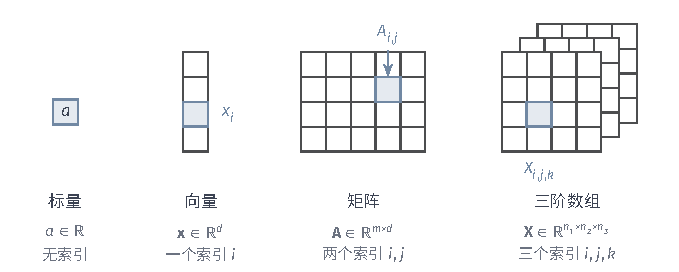
\includegraphics[width=112mm]{figures/00-shared/mathematical-preliminaries-upper/02-linear-spaces/tikz/comprehension-additions/scalar-vector-matrix-tensor.pdf}
  \caption{标量、向量、矩阵与三阶数组的区别。每个面板用蓝色标出一个数：标量本身就是这个数，向量用一个索引$i$定位，矩阵用行列两个索引$i,j$定位，三阶数组再加一个索引$k$选择切片。索引个数称为阶，各轴长度组成形状。}
  \label{fig:ls-scalar-vector-matrix-tensor}
\end{figure}

两个同形数组按位置逐项相加、数乘，规则与向量、矩阵完全相同；两个数组能否相加，仍要求形状相同、对应轴的含义相同。使用多维数组时，须先说清每条轴记录什么：同一个$b\times\ell\times d$数组，若把第二、三轴的含义弄反，后续的每一次汇总都会汇总错的轴。

\subsection{张量的运算}
\label{sec:ls-tensor-operations}

多轴数组的运算按对轴的作用分成三类。轴置换与形状重整只改变元素记录在哪条轴、哪个位置上，不改变数值，也不求和。张量积和它的矩阵形式Kronecker积把多个因子的轴全部保留下来，组合成轴更多的数组。缩约则反过来，指定一对或几对轴对齐相乘后求和，把数组汇总成更低阶的数组。

\subsubsection{轴置换}
\label{sec:ls-tensor-reshaping}
\phantomsection
\label{sec:linear-algebra-tensors-structured-operations}

\term{维度重排}（permutation of axes）按给定顺序调换轴的位置，元素跟随自己的索引移动。计算时先写出新旧索引的对应，再按对应搬运元素。例如把$\bm X\in\mathbb R^{b\times\ell\times d}$的第二、三轴互换，得到$\bm Y\in\mathbb R^{b\times d\times\ell}$，
\[
 y_{i,k,j}=x_{i,j,k}.
\]
第一个轴保持原位，每个样本的切片被转置：$\bm Y_{i,:,:}=(\bm X_{i,:,:})^\top$。下面取一个具体的小数组。
\begin{example}[交换后两条轴]
\label{ex:ls-axis-swap}
给定：$b=1$、$\ell=2$、$d=3$，唯一的样本切片为$\bm X_{1,:,:}=\left[\begin{smallmatrix}1&2&3\\4&5&6\end{smallmatrix}\right]$。
计算：按$y_{1,k,j}=x_{1,j,k}$搬运元素，例如$y_{1,3,2}=x_{1,2,3}=6$，得到
\[
 \bm Y_{1,:,:}=\begin{bmatrix}1&4\\2&5\\3&6\end{bmatrix}.
\]
结论：$\bm Y\in\mathbb R^{1\times3\times2}$，它的样本切片正是原切片的转置。
\end{example}
矩阵的转置是两个轴时唯一的非平凡轴置换。轴的含义跟着轴走，不因位置改变而改变：$\bm Y$的第二轴仍是特征，第三轴仍是位置。

\subsubsection{形状重整与向量化}

\term{形状重整}（reshape）先按指定的遍历顺序把全部元素读成一个数列，再把这个数列按同样的顺序装入另一形状；它只要求元素总数相同。计算分两步：读出、装入。下面的例子比较按行重整与转置。
\begin{example}[按行重整与转置的区别]
\label{ex:ls-reshape-vs-transpose}
给定：$\bm A=\left[\begin{smallmatrix}1&2&3\\4&5&6\end{smallmatrix}\right]$，目标形状为$3\times2$。
计算：按行读出得数列$1,2,3,4,5,6$，再按行装入$3\times2$数组，得到
\[
 \bm R=\begin{bmatrix}1&2\\3&4\\5&6\end{bmatrix},
 \qquad\text{而}\qquad
 \bm A^\top=\begin{bmatrix}1&4\\2&5\\3&6\end{bmatrix}.
\]
结论：$\bm R$与$\bm A^\top$形状相同、所含的数相同，排列却不同。
\end{example}
所以重整不能只给目标形状，还要给遍历顺序；形状相同也不能说明完成了轴交换。图~\ref{fig:vol1-add-linear-transpose-reshape}把两种结果并排放置。
\begin{figure}[!htb]
  \centering
  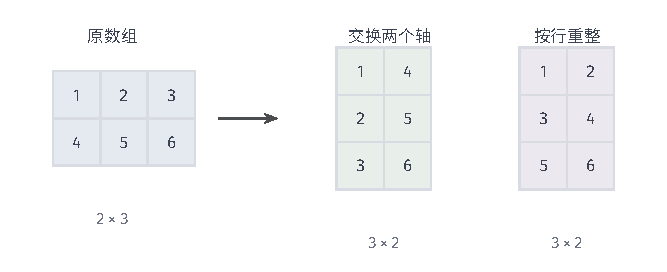
\includegraphics[width=112mm]{figures/00-shared/mathematical-preliminaries-upper/02-linear-spaces/tikz/comprehension-additions/linear-transpose-reshape.pdf}
  \caption{轴交换与按行重整。原数组两行为$(1,2,3)$与$(4,5,6)$；中图转置后两列分别保留原来的两行，右图则把按行读取的数列$1,2,3,4,5,6$依次装入$3\times2$数组。数字及其排列由正文示例直接给出。}
  \label{fig:vol1-add-linear-transpose-reshape}
\end{figure}

形状重整中最常用的一种，是把矩阵按列堆叠成一个长列向量，称为\term{向量化}（vectorization）：
\[
 \operatorname{vec}(\bm A)=(a_{1,1},\ldots,a_{m,1},a_{1,2},\ldots,a_{m,2},\ldots,a_{1,n},\ldots,a_{m,n})^\top,
\]
$m\times n$矩阵的元素$a_{i,j}$位于一维索引$i+(j-1)m$。例如上面的$\bm A$给出$\operatorname{vec}(\bm A)=(1,4,2,5,3,6)^\top$，其中$a_{2,3}=6$位于第$2+(3-1)\cdot2=6$个位置。

多维数组也可以按轴重整成矩阵，称为矩阵展开（unfolding）：把一部分轴合并成行索引，其余轴合并成列索引。例如把$\bm X\in\mathbb R^{b\times\ell\times d}$的前两轴合并为行，得到$b\ell\times d$矩阵，每行是一个样本在一个位置上的特征。选哪些轴合并，决定展开结果的形状，也决定后续乘积汇总哪个轴。

\subsubsection{张量积}
\label{sec:ls-tensor-products}
\phantomsection
\label{sec:linear-algebra-joint-operations}

两个向量的全部两两乘积排成一个数组，就是它们的张量积。设$\bm x\in\mathbb R^m$、$\bm y\in\mathbb R^n$，\term{张量积}（tensor product）$\bm x\otimes\bm y$是$m\times n$数组，
\[
 (\bm x\otimes\bm y)_{i,j}=x_i y_j.
\]
写成矩阵，$\bm x\otimes\bm y=\bm x\bm y^\top$，正是分块乘法式~\eqref{eq:ls-product-outer-sum}中“一列乘一行”的矩阵。每个因子各占结果的一条轴，下面称为一个槽位。三个向量的张量积$(\bm x\otimes\bm y\otimes\bm z)_{i,j,k}=x_i y_j z_k$保留三个槽位，多重张量积按同样规则逐槽位相乘。下面计算两个二维向量的张量积。
\begin{example}[两个二维向量的张量积]
\label{ex:ls-tensor-product-two-vectors}
给定：$\bm x=(1,2)^\top$，$\bm y=(3,-1)^\top$。
计算：
\[
 \bm x\otimes\bm y=\begin{pmatrix}1\cdot3&1\cdot(-1)\\2\cdot3&2\cdot(-1)\end{pmatrix}=\begin{pmatrix}3&-1\\6&-2\end{pmatrix}.
\]
结论：第$i$行是$x_i\bm y^\top$，所以每一行都是$\bm y^\top$的倍数；同理，每一列都是$\bm x$的倍数。
\end{example}
图~\ref{fig:ls-tensor-product-slots}展示张量积怎样保留两个因子的槽位。
\begin{figure}[htbp]
  \centering
  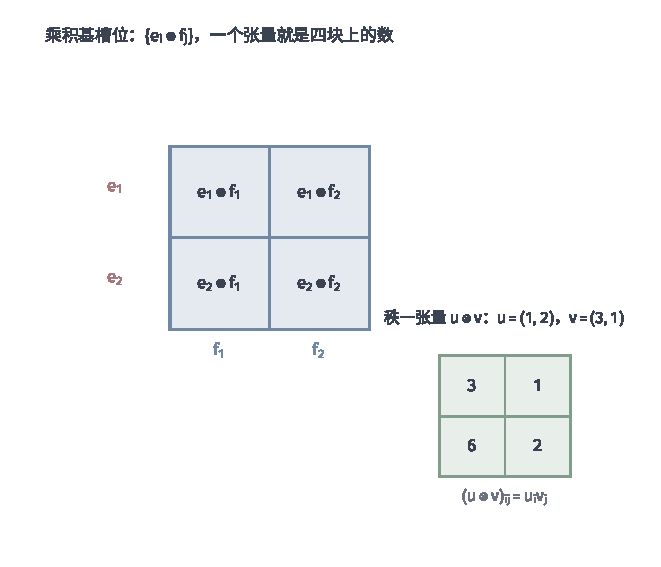
\includegraphics[width=112mm]{figures/00-shared/mathematical-preliminaries-upper/02-linear-spaces/matplotlib/ls-tensor-product-slots/ls-tensor-product-slots.pdf}
  \caption{张量积并排保留两个因子的槽位。左：$\bm u\in\mathbb R^2$、$\bm v\in\mathbb R^3$。右：$\bm u\otimes\bm v$排成$2\times3$网格，每行由$\bm v$方向复制并按$u_i$缩放；它是简单张量，数值由$\bm u=(1,0.6)$、$\bm v=(1,0.5,0.2)$直接相乘得到，是教学构造。}
  \label{fig:ls-tensor-product-slots}
\end{figure}

形如$\bm x\otimes\bm y$的数组称为\term{简单张量}（simple tensor）。由示例~\ref{ex:ls-tensor-product-two-vectors}的结论，简单张量的各行都是同一个向量的倍数。并非每个二阶数组都是简单张量，下面是一个反例。
\begin{example}[反例：单位矩阵不是简单张量]
\label{ex:ls-identity-not-simple}
给定：$\bm I_2$，它的两行为$(1,0)$与$(0,1)$。
验证：若$\bm I_2=\bm x\otimes\bm y$，则两行分别是$x_1\bm y^\top$与$x_2\bm y^\top$。两行都非零，所以$x_1,x_2\neq0$，两行都是$\bm y^\top$的非零倍数，从而彼此成比例。但$(1,0)$与$(0,1)$不成比例。
结论：$\bm I_2$不能写成任何$\bm x\otimes\bm y$，它不是简单张量。
\end{example}
不过，每个$m\times n$数组$\bm T$都是简单张量的和，
\[
 \bm T=\sum_{i,j}t_{i,j}\,\bm e_i\otimes\bm f_j,
\]
其中$\bm e_i$、$\bm f_j$分别是$\mathbb R^m$与$\mathbb R^n$的标准坐标向量，$\bm e_i\otimes\bm f_j$只在位置$(i,j)$为$1$。

张量积的用处，是把同时依赖两组输入的读取化为对单个数组的线性读取。设实值函数$B(\bm x,\bm y)$对$\bm x$、$\bm y$分别保持线性组合（称为双线性）。把$\bm x=\sum_ix_i\bm e_i$、$\bm y=\sum_jy_j\bm f_j$代入，按两次线性展开，
\[
 B(\bm x,\bm y)=\sum_{i,j}x_iy_j\,B(\bm e_i,\bm f_j)=\sum_{i,j}g_{i,j}(\bm x\otimes\bm y)_{i,j}
 =\langle\bm G,\bm x\otimes\bm y\rangle_{\mathrm F},
\]
其中$g_{i,j}=B(\bm e_i,\bm f_j)$。所以双线性读取由一张固定的系数表$\bm G$决定，并且它对数组$\bm x\otimes\bm y$是线性的。以欧氏内积$B(\bm x,\bm y)=\bm x^\top\bm y$（$m=n$）为例，$g_{i,j}=\langle\bm e_i,\bm e_j\rangle$，即$\bm G=\bm I$，读取就是把$\bm x\otimes\bm y$的对角线加起来。

二阶张量与矩阵是同一组数的两种记录：张量强调槽位来自哪一组输入，矩阵强调行列在乘法中的角色。

\subsubsection{Kronecker积}

两个矩阵分别作用在两条轴上时，联合作用可以写成一张大矩阵。对$\bm A\in\mathbb R^{m\times n}$、$\bm B\in\mathbb R^{p\times q}$，定义Kronecker积
\begin{equation}
 \bm A\otimes\bm B
 =\begin{bmatrix}
  A_{1,1}\bm B&\cdots&A_{1,n}\bm B\\
  \vdots&\ddots&\vdots\\
  A_{m,1}\bm B&\cdots&A_{m,n}\bm B
 \end{bmatrix}\in\mathbb R^{mp\times nq}.
 \label{eq:linear-algebra-kronecker-product}
\end{equation}
计算时把$\bm A$的每个元素$A_{i,j}$替换成块$A_{i,j}\bm B$。下面计算一个二阶的例子。
\begin{example}[两个二阶矩阵的Kronecker积]
\label{ex:ls-kronecker-two-by-two}
给定：$\bm A=\left[\begin{smallmatrix}1&2\\3&4\end{smallmatrix}\right]$，$\bm B=\left[\begin{smallmatrix}0&1\\1&0\end{smallmatrix}\right]$。
计算：
\[
 \bm A\otimes\bm B
 =\begin{bmatrix}
  1\cdot\bm B&2\cdot\bm B\\
  3\cdot\bm B&4\cdot\bm B
 \end{bmatrix}
 =\begin{bmatrix}0&1&0&2\\1&0&2&0\\0&3&0&4\\3&0&4&0\end{bmatrix}.
\]
结论：$\bm A\otimes\bm B$是$4\times4$矩阵，四个$2\times2$块依次是$\bm B$的$1,2,3,4$倍。
\end{example}
图~\ref{fig:ls-kronecker-block-structure}用另一组数展示这种逐元素替换的分块结构。
\begin{figure}[htbp]
  \centering
  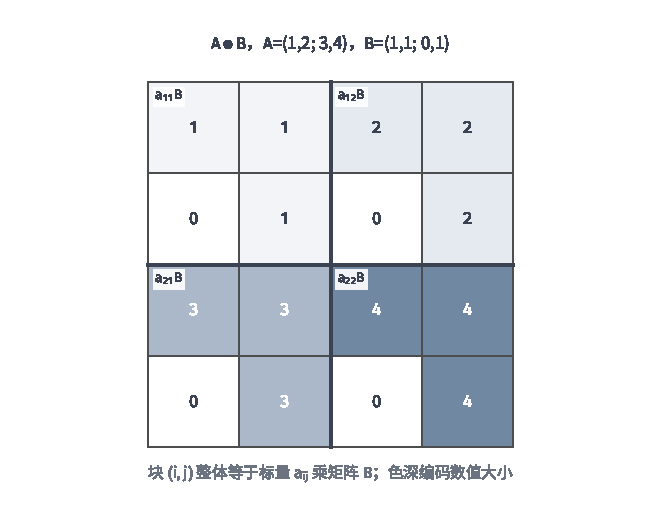
\includegraphics[width=112mm]{figures/00-shared/mathematical-preliminaries-upper/02-linear-spaces/matplotlib/ls-kronecker-block-structure/ls-kronecker-block-structure.pdf}
  \caption{Kronecker积的分块结构。上：$\bm A=\bigl(\begin{smallmatrix}1&2\\3&4\end{smallmatrix}\bigr)$、$\bm B=\bigl(\begin{smallmatrix}10&20\\30&40\end{smallmatrix}\bigr)$。下：$\bm A\otimes\bm B$是把$\bm A$的每个元素替换为该元素乘$\bm B$得到的$4\times4$分块矩阵，块边界用白线强调。数值由定义直接计算，是教学例。}
  \label{fig:ls-kronecker-block-structure}
\end{figure}

两个列向量按式~\eqref{eq:linear-algebra-kronecker-product}相乘，得到$mn$维长向量$(x_1\bm y^\top,\ldots,x_m\bm y^\top)^\top$，它正是把$m\times n$数组$\bm x\otimes\bm y$按行读出的结果。两种用法记录的是同一组数，只差一次按行读出，所以同一个记号$\otimes$不会引起混淆。例如$(1,2)^\top\otimes(3,-1)^\top=(3,-1,6,-2)^\top$，与示例~\ref{ex:ls-tensor-product-two-vectors}中的数组按行读出的结果相同。

\subsubsection{张量缩约}
\label{sec:ls-tensor-contraction}

张量积把槽位全部保留；缩约则沿指定的轴汇总。计算时选定一对或几对尺寸相同的轴，让每对轴共用同一个求和索引，逐项相乘后对这些索引求和；被求和的轴消失，其余轴保留，按原次序组成输出的形状。写出索引，就能检查哪些轴被消去、哪些轴应当保留，下面用两个例子说明这种检查。
\begin{example}[两种缩约的输出形状]
\label{ex:ls-contraction-shapes}
给定：（1）$\bm A\in\mathbb R^{m\times d\times r}$与$\bm B\in\mathbb R^{d\times n\times r}$；（2）$\bm X\in\mathbb R^{b\times\ell\times d}$与$\bm W\in\mathbb R^{d\times h}$。
计算：（1）让$\bm A$的第二轴与$\bm B$的第一轴共用索引$k$，两者的第三轴共用索引$s$，
\[
 c_{i,j}=\sum_{k=1}^d\sum_{s=1}^r a_{i,k,s}b_{k,j,s}.
\]
（2）让$\bm X$的最后一轴与$\bm W$的第一轴共用索引$k$，
\[
 z_{i,j,t}=\sum_{k=1}^d x_{i,j,k}w_{k,t}.
\]
结论：（1）同时消去$k$与$s$两对轴，保留$i,j$，输出为$m\times n$矩阵。（2）只消去$k$，保留$i,j,t$，输出形状为$b\times\ell\times h$：每个样本、每个位置上的$d$维特征都乘了同一个矩阵$\bm W$。
\end{example}
图~\ref{fig:ls-tensor-contraction}沿一对选中的轴求和并保留其余轴。
\begin{figure}[htbp]
  \centering
  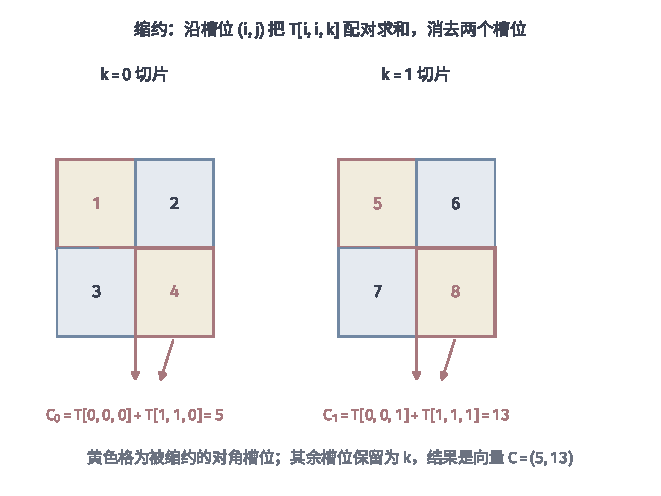
\includegraphics[width=112mm]{figures/00-shared/mathematical-preliminaries-upper/02-linear-spaces/matplotlib/ls-tensor-contraction/ls-tensor-contraction.pdf}
  \caption{张量缩约沿选中的一对轴求和、保留其余轴。左：二阶张量按行和列着色；选中列轴（虚线箭头）沿列求和，输出对每行汇总为一个值。右：缩约后得到$3$个输出，分别对应原矩阵三行的行和，颜色由红（小）经黄到蓝（大）。张量与数值均为解析教学例。}
  \label{fig:ls-tensor-contraction}
\end{figure}

前两节的几种运算都是缩约：
\begin{itemize}
 \item 内积$\sum_jx_jy_j$缩约两个向量唯一的一对轴，输出标量；
 \item 矩阵乘法$\sum_\ell a_{i,\ell}b_{\ell,j}$只消去左因子的列轴与右因子的行轴这一对；
 \item 迹$\sum_iA_{i,i}$把同一个矩阵的行轴与列轴对齐到同一索引后求和；
 \item Frobenius内积$\sum_{i,j}a_{i,j}b_{i,j}$同时缩约两对轴。
\end{itemize}

\subsection{张量运算的性质}
\label{sec:ls-tensor-operation-properties}

使用上一小节的运算时，须知道哪些操作可以撤销、括号怎样移动、Kronecker积怎样与普通矩阵乘法配合，以及缩约何时可以分开计算。本小节按运算整理，最后用一张表汇总各种“乘法”的形状条件。

\subsubsection{重排的性质}

\paragraph{可逆性}
目标形状与遍历顺序固定后，轴置换、形状重整与向量化都把一个数组一一对应到另一个数组，逆操作恢复原数组：转置再转置、按逆置换换回、按原顺序装回。例如$\operatorname{vec}$的逆操作把长度为$mn$的向量依次每$m$个一列装回$m\times n$矩阵。所以重排保留全部信息。

\paragraph{线性}
\[
 \operatorname{vec}(a\bm A+b\bm B)=a\operatorname{vec}(\bm A)+b\operatorname{vec}(\bm B),
\]
轴置换与形状重整同样满足这一性质：它们只搬动元素，逐项的加法与数乘搬到新位置后不变。

\paragraph{与矩阵乘法的关系}
转置与乘法有整齐的规则$(\bm A\bm B)^\top=\bm B^\top\bm A^\top$；一般的形状重整与乘法没有这样的关系。重整以后，矩阵每一行、每一列汇集的元素都变了，依赖行列结构的乘积、迹与行列式一般随之改变。下面的反例把示例~\ref{ex:ls-reshape-vs-transpose}中的$\bm R$误当作$\bm A^\top$使用。
\begin{example}[反例：重整不能代替转置]
\label{ex:ls-reshape-breaks-product}
给定：$\bm A=\left[\begin{smallmatrix}1&2&3\\4&5&6\end{smallmatrix}\right]$，以及按行重整得到的$\bm R=\left[\begin{smallmatrix}1&2\\3&4\\5&6\end{smallmatrix}\right]$。
计算：由示例~\ref{ex:ls-gram-product-symmetric}，$\bm A\bm A^\top=\left[\begin{smallmatrix}14&32\\32&77\end{smallmatrix}\right]$；而
\[
 \bm A\bm R=\begin{bmatrix}1+6+15&2+8+18\\4+15+30&8+20+36\end{bmatrix}=\begin{bmatrix}22&28\\49&64\end{bmatrix}.
\]
结论：$\bm R$与$\bm A^\top$形状相同、所含的数相同，两个乘积的迹却分别为$14+77=91$与$22+64=86$。
\end{example}
把存储格式的改变当成计算效果，是这里最常见的错误。

\subsubsection{张量积的性质}

\paragraph{对每个因子线性}
\[
 (a\bm x)\otimes\bm y=\bm x\otimes(a\bm y)=a(\bm x\otimes\bm y),\qquad
 (\bm x+\bm x')\otimes\bm y=\bm x\otimes\bm y+\bm x'\otimes\bm y,
\]
对第二个因子的加法同样分配。每个元素$x_iy_j$对$x_i$和$y_j$分别线性，逐项验证即得。

\paragraph{结合律}
\[
 (\bm x\otimes\bm y)\otimes\bm z=\bm x\otimes(\bm y\otimes\bm z),
\]
两边的$(i,j,k)$元素都是$x_iy_jz_k$。

\paragraph{交换槽位是转置}
\[
 \bm y\otimes\bm x=(\bm x\otimes\bm y)^\top,
\]
因为$\bm x\otimes\bm y$的$(i,j)$元素$x_iy_j$也是$\bm y\otimes\bm x$的$(j,i)$元素。所以一般$\bm x\otimes\bm y\neq\bm y\otimes\bm x$，两者相差一次轴置换。

\paragraph{Frobenius配对与范数分离}
\[
 \langle\bm x\otimes\bm y,\bm x'\otimes\bm y'\rangle_{\mathrm F}
 =\langle\bm x,\bm x'\rangle\langle\bm y,\bm y'\rangle,
 \qquad
 \lVert\bm x\otimes\bm y\rVert_{\mathrm F}=\lVert\bm x\rVert_2\,\lVert\bm y\rVert_2.
\]
第一式来自$\sum_{i,j}x_iy_jx'_iy'_j=(\sum_ix_ix'_i)(\sum_jy_jy'_j)$；第二式在第一式中取$\bm x'=\bm x$、$\bm y'=\bm y$后开平方。下面在示例~\ref{ex:ls-tensor-product-two-vectors}的数组上核对第二式。
\begin{example}[张量积范数的数值核对]
\label{ex:ls-tensor-product-norm-check}
给定：$\bm x=(1,2)^\top$，$\bm y=(3,-1)^\top$，$\bm x\otimes\bm y=\left(\begin{smallmatrix}3&-1\\6&-2\end{smallmatrix}\right)$。
计算：$\lVert\bm x\rVert_2=\sqrt5$，$\lVert\bm y\rVert_2=\sqrt{10}$；直接求Frobenius范数，
\[
 \lVert\bm x\otimes\bm y\rVert_{\mathrm F}=\sqrt{3^2+(-1)^2+6^2+(-2)^2}=\sqrt{50}.
\]
结论：$\sqrt5\cdot\sqrt{10}=\sqrt{50}=5\sqrt2$，两种算法一致。
\end{example}

\paragraph{与楔积的联系}
矩阵一节的楔积也可以由张量积经反对称化得到：$\bm x\wedge\bm y$对应$\bm x\otimes\bm y-\bm y\otimes\bm x$，交换$\bm x,\bm y$时它变号。这里只指出联系，楔积的规则不依赖张量积。

\subsubsection{Kronecker积的性质}
\label{sec:ls-kronecker-products}

\paragraph{分别作用于两个槽位}
\[
 (\bm A\otimes\bm B)(\bm x\otimes\bm y)=(\bm A\bm x)\otimes(\bm B\bm y).
\]
按分块乘法，左侧第$i$块为$\sum_jA_{i,j}\bm B(x_j\bm y)=(\sum_jA_{i,j}x_j)\bm B\bm y=(\bm A\bm x)_i\,\bm B\bm y$，正是右侧的第$i$块。第一个槽位只经过$\bm A$，第二个槽位只经过$\bm B$，两个作用并行而不串联；矩阵乘法则把前后两次作用串成一条链。

\paragraph{混合乘积}
当$\bm A\bm C$与$\bm B\bm D$分别有定义时，
\begin{equation}
 (\bm A\otimes\bm B)(\bm C\otimes\bm D)
 =(\bm A\bm C)\otimes(\bm B\bm D).
 \label{eq:matrix-analysis-kronecker-mixed-product}
\end{equation}
按分块乘法，左侧的块$(i,k)$为$\sum_j(A_{i,j}\bm B)(C_{j,k}\bm D)=(\sum_jA_{i,j}C_{j,k})\bm B\bm D=(\bm A\bm C)_{i,k}\bm B\bm D$，恰是右侧的块。上一条是$\bm C,\bm D$各只有一列的情形。

\paragraph{转置}
\[
 (\bm A\otimes\bm B)^\top=\bm A^\top\otimes\bm B^\top.
\]
分块矩阵转置时，块的位置交换，每块各自转置，所以第$(j,i)$块为$A_{i,j}\bm B^\top$，正是$\bm A^\top\otimes\bm B^\top$的第$(j,i)$块。

\paragraph{逆}
\[
 (\bm A\otimes\bm B)^{-1}=\bm A^{-1}\otimes\bm B^{-1}\qquad(\bm A,\bm B\text{都可逆}).
\]
由混合乘积，$(\bm A\otimes\bm B)(\bm A^{-1}\otimes\bm B^{-1})=(\bm A\bm A^{-1})\otimes(\bm B\bm B^{-1})=\bm I\otimes\bm I=\bm I$，另一侧同理。

\paragraph{迹}
\[
 \operatorname{tr}(\bm A\otimes\bm B)=\operatorname{tr}\bm A\,\operatorname{tr}\bm B\qquad(\bm A,\bm B\text{都是方阵}).
\]
只有对角块$A_{i,i}\bm B$的对角元落在主对角线上，所以迹为$\sum_iA_{i,i}\operatorname{tr}\bm B=\operatorname{tr}\bm A\,\operatorname{tr}\bm B$。

\paragraph{向量化恒等式}
对$\bm A\in\mathbb R^{p\times m}$、$\bm X\in\mathbb R^{m\times n}$、$\bm B\in\mathbb R^{n\times q}$，
\begin{equation}
 \operatorname{vec}(\bm A\bm X\bm B)
 =(\bm B^\top\otimes\bm A)\operatorname{vec}(\bm X).
 \label{eq:matrix-analysis-vec-kronecker}
\end{equation}
比较两侧输出的第$j$段（长度为$p$）。左侧是$\bm A\bm X\bm B$的第$j$列，$\bm A\bm X\bm B_{:,j}=\sum_kB_{k,j}\bm A\bm X_{:,k}$。右侧矩阵的第$j$块行为$(B_{1,j}\bm A,\ldots,B_{n,j}\bm A)$，与$\operatorname{vec}(\bm X)$的各段$\bm X_{:,1},\ldots,\bm X_{:,n}$相乘，也得到$\sum_kB_{k,j}\bm A\bm X_{:,k}$。逐元素写出，两侧$(i,j)$位置的元素都是$\sum_{\ell=1}^m\sum_{k=1}^n A_{i,\ell}X_{\ell,k}B_{k,j}$。

固定$\bm A,\bm B$后，这一恒等式把“两侧同时乘矩阵”写成对长向量$\operatorname{vec}(\bm X)$乘一张矩阵，从而把关于未知矩阵的方程化成普通线性方程组；第~\ref{chap:linear-equations-and-optimization}章求解矩阵方程时将用到它。

\subsubsection{缩约的性质}

\paragraph{线性}
固定配对数组后，缩约对被作用数组线性：把被作用数组换成$a\bm X+b\bm X'$，输出变为$a$倍与$b$倍两个输出之和。这是因为每个输出元素都是被作用数组元素以固定系数作的加权和。

\paragraph{求和次序可交换}
多对轴的缩约是有限和，结果与先消哪一对轴无关。例如示例~\ref{ex:ls-contraction-shapes}中的$c_{i,j}$可以先对$s$求和得到中间数组，再对$k$求和，也可以反过来。

\paragraph{简单张量系数可分离}
一次读取同时依赖三组向量$\bm x\in\mathbb R^m$、$\bm y\in\mathbb R^n$、$\bm z\in\mathbb R^p$时，若系数数组是简单张量$\bm a\otimes\bm b\otimes\bm c$，则
\begin{equation}
 \left\langle\bm a\otimes\bm b\otimes\bm c,
 \bm x\otimes\bm y\otimes\bm z\right\rangle_{\mathrm F}
 =(\bm a^\top\bm x)(\bm b^\top\bm y)(\bm c^\top\bm z),
 \label{eq:linear-algebra-rank-one-contraction}
\end{equation}
因为$\sum_{i,j,k}a_ib_jc_kx_iy_jz_k=(\sum_ia_ix_i)(\sum_jb_jy_j)(\sum_kc_kz_k)$：三重求和分离成三个内积的乘积，计算量从$mnp$项降到$m+n+p$项。下面用一组小数值核对。
\begin{example}[简单张量系数的分离计算]
\label{ex:ls-rank-one-contraction-check}
给定：$\bm a=(1,2)^\top$、$\bm b=(3,-1)^\top$、$\bm c=(2,1)^\top$，$\bm x=(2,1)^\top$、$\bm y=(1,1)^\top$、$\bm z=(1,-1)^\top$，这里$m=n=p=2$。
计算：三个内积依次为
\[
 \begin{gathered}
 \bm a^\top\bm x=1\cdot2+2\cdot1=4,\qquad
 \bm b^\top\bm y=3\cdot1+(-1)\cdot1=2,\\
 \bm c^\top\bm z=2\cdot1+1\cdot(-1)=1.
 \end{gathered}
\]
结论：由式~\eqref{eq:linear-algebra-rank-one-contraction}，读取等于$4\cdot2\cdot1=8$；直接展开三重求和要累加$2^3=8$项乘积，结果同样是$8$。
\end{example}

\paragraph{非线性操作不是缩约}
$\operatorname{softmax}$、逐元素非线性等操作不属于缩约。一个模型即使由缩约和这些操作交替组成，固定系数时每一步缩约的线性也不代表整体线性。

\subsubsection{各种乘积的形状}

本章出现了好几种“乘法”，它们的区别在于对索引做什么。表~\ref{tab:linear-algebra-products-and-shapes}汇总它们的形状条件与索引作用。

\begin{table*}[htbp]
 \centering\small
 \begin{tabularx}{\linewidth}{@{}lXX@{}}
  \toprule
  运算 & 形状条件与输出 & 索引作用\\
  \midrule
  $\langle\bm x,\bm y\rangle$ & 两个$n$维向量，输出标量 & 配对后汇总\\
  $\bm A\bm B$ & $(m\times n)(n\times p)\to m\times p$ & 汇总共同索引\\
  $\bm A\odot\bm B$ & 同为$m\times n$，输出仍为$m\times n$ & 同位置相乘，不求和\\
  $\bm x\otimes\bm y$ & $m$维与$n$维向量$\to m\times n$ & 保留两条轴，不求和\\
  $\bm A\otimes\bm B$ & $(m\times n)$与$(p\times q)\to(mp)\times(nq)$ & 保留两组成对索引\\
  缩约 & 被缩约的各对轴尺寸相同 & 消去指定轴，保留其余轴\\
  \bottomrule
 \end{tabularx}
 \caption{相乘符号对应不同操作。先检查消去哪些索引，再判断其线性性和输出含义。}
 \label{tab:linear-algebra-products-and-shapes}
\end{table*}

% 第4章：本章小结。

\section{本章小结}
\label{sec:ls-operations-summary}

本章按定位一个数所需的索引个数，依次处理向量、矩阵与张量，并对每种运算交代输入条件、输出形状和可用的规则。向量的加法与数乘合成线性组合；内积把两个向量配成一个数，范数用四条公理统一各种误差口径，由内积给出的欧氏范数还满足平行四边形恒等式。

矩阵乘积来自两次加权求和的复合，满足结合律与分配律，却不满足交换律与消去律；逆矩阵撤销一次乘法，矩阵幂记录反复作用。迹、行列式与矩阵范数把矩阵读成一个数：行列式是有向体积的缩放倍数，诱导范数是最坏情形的放大倍数。张量把索引推广到任意多个：重排只改变元素位置，张量积保留全部槽位，缩约沿指定的轴求和，内积、矩阵乘积与迹都是缩约的特例。

本章只把这些数组当作具体的数表。第~\ref{chap:linear-representation}章接着追问它们记录的是什么：同一个对象换一组方向后坐标怎样改变，矩阵怎样记录线性映射，一般空间中的夹角与正交怎样讨论。矩阵反复作用的走向与误差的放大留给第~\ref{chap:linear-analysis}章，方程怎样求解留给第~\ref{chap:linear-equations-and-optimization}章。

